\chapter{Taxonomy of Images and Algorithms}
\label{chap:image.algorithms.taxonomy}

In this thesis, we researched how to apply all those new generic facilities from the C++ language into the Image
processing area. This allows us to test them in a practical way on our predilection area while remembering our past
work, both success and failures in this matter. However, as we saw in the previous chapter~\ref{chap:genericity},
birthing concepts from code is something that is done in an emerging way. Henceforth, the first work will be to do an
inventory of all existing image algorithms as well as an inventory of all image processing algorithms (both basic and
more complex) we can think of. This way, we will notice behavior patterns emerging from similar image types or similar
algorithms. First we will study how to extract behavioral pattern from an algorithm in order to refine it into one or
multiple concepts. We will then study the set theory behind images types, their conjunctions, disjunctions and the
implications. We will then study behavioral pattern related to algorithms, as well as their specific problematics
related to heterogeneous computation. Finally, we will propose show the result of this emerging inventory in the form of
a taxonomy indexing a framework of concepts about image processing.

\section{Rewriting an algorithm to extract a concept}
\label{sec:rewriting}

\subsection{Gamma correction}
\label{subsec:gamma}

Let us take the gamma correction algorithm as an example. The naive way to write this algorithm can be:

\begin{minted}[linenos]{C++}
template <class Image>
void gamma_correction(Image& ima, double gamma)
{
  const auto gamma_corr = 1.f / gamma;

  for (int x = 0; x < ima.width(); ++x)
    for (int y = 0; y < ima.height(); ++y)
    {
      ima(x, y).r = 256.f * std::pow(ima(x, y).r / 256.f, gamma_corr);
      ima(x, y).g = 256.f * std::pow(ima(x, y).g / 256.f, gamma_corr);
      ima(x, y).b = 256.f * std::pow(ima(x, y).b / 256.f, gamma_corr);
    }
}
\end{minted}

\noindent This algorithm here performs the transformation correctly but it also makes a lot of hypothesis. Firstly, we
suppose that we can write in the image via the \texttt{=} operator (l.9-11): it may not be true if the image is sourced
from a generator function. Secondly, we suppose that we have a 2D image via the double loop (l.6-7). Finally, we suppose
we are operating on 8bits range (0-255) RGB via \texttt{'.r'}, \texttt{'.g'}, \texttt{'.b'} (l.9-11). Those hypothesis
are unjustified. Intrinsically, all we want to say is \blockquote{\emph{For each value of \texttt{ima}, apply a gamma
    correction on it.}}. Let us proceed to make this algorithm the most generic possible by lifting those unjustified
constraints one by one.



\paragraph{Lifting RGB constraint:}
First, we get rid of the 8bits color range (0-255) RGB format requirement. The loops become:

\begin{minted}{C++}
  using value_t = typename Image::value_type;

  const auto gamma_corr = 1.f / gamma;
  const auto max_val = std::numeric_limits<value_t>::max();

  for(int x = 0; x < ima.width(); ++x)
    for(int y = 0; y < ima.height(); ++y)
      ima(x, y) = max_val * std::pow(ima(x, y) / max_val, gamma_corr);
\end{minted}

\noindent By lifting this constraint, we now require the type Image to define a nested type \texttt{Image::value\_type}
(returned by \texttt{ima(x, y)}) on which \texttt{std::numeric\_limits} and \texttt{std::pow} are defined. This way the
compiler will be able to check the types at compile-time and emit warning and/or errors in case it detects
incompatibilities. We are also able to detect it beforehand using a \texttt{static\_assert} for instance.1



\paragraph{Lifting bi-dimensional constraint:}
Here we need to introduce a new abstraction layer, the \emph{pixel}. A \emph{pixel} is a couple $(point, value)$. The
double loop then becomes:

\begin{minted}{C++}
  for (auto&& val : ima.values())
    val = max_val * std::pow(val / max_val, gamma_corr);
\end{minted}

\noindent This led to us requiring that the type \emph{Image} requires to provide a method \texttt{Image::pixels()} that
returns \emph{something} we can iterate on with a range-for loop: this \emph{something} is a \emph{Range} of
\emph{Pixel}. This \emph{Range} is required to behave like an \emph{iterable}: it is an abstraction that provides a way
to browse all the elements one by one. The \emph{Pixel} is required to provide a method \texttt{Pixel::value()} that
returns a \emph{Value} which is \emph{Regular}~(see \cref{term:regular}). Here, we use \texttt{auto\&\&} instead of
\texttt{auto\&} to allow the existence of proxy iterator (think of \texttt{vector<bool>}). Indeed, we may be iterating
over a lazy-computed view~\cref{chap:image_views}.



\paragraph{Lifting writability constraint:}
Finally, the most subtle one is the requirement about the \emph{writability} of the image. This requirement can be
expressed directly via the new C++20 syntax for \emph{concepts}. All we need to do is changing the template declaration
by:

\begin{minted}{C++}
template <WritableImage Image>
\end{minted}

\noindent In practice the C++ keyword \texttt{const} is not enough to express the \emph{constness} or the
\emph{mutability} of an image. Indeed, we can have an image whose pixel values are returned by computing $cos(x+y)$ (for
a 2D point). Such an image type can be instantiated as \emph{non-const} in C++ but the values will not be
\emph{mutable}: this type will not model the \emph{WritableImage} concept.



\paragraph{Final version}

\begin{minted}{C++}
template <WritableImage Image>
void gamma_correction(Image& ima, double gamma)
{
  using value_t = typename Image::value_type;

  const auto gamma_corr = 1 / gamma;
  const auto max_val = numeric_limits<value_t>::max();

  for (auto&& pix : ima.pixels())
    pix.value() = std::pow((max_val * pix.value()) / max_val, gamma_corr);
}
\end{minted}

\noindent When re-writing a lot of algorithms this way: lifting constraints by requiring behavior instead, we are able
to deduce what our \emph{concepts} needs to be. The real question for a \emph{concept} is: \blockquote{\emph{what
    behavior should be required?}}



\subsection{Dilation algorithm}
\label{subsec:dilation}

To show the versatility of this approach, we will now attempt to deduces the requirements necessary to write a classical
\emph{dilate} algorithm. First let us start with a naive implementation:

\begin{minted}[linenos]{C++}
template <class InputImage, class OutputImage>
void dilate(const InputImage& input_ima, OutputImage& output_ima)
{
  assert(input_ima.height() == output_ima.height()
    && input_ima.width() == output_ima.width());

  for (int x = 2; x < input_ima.width() - 2; ++x)
    for (int y = 2; y < input_ima.height() - 2; ++y)
    {
      output_ima(x, y) = input_ima(x, y)
      for (int i = x - 2; i <= x + 2; ++i)
        for (int j = y - 2; j <= y + 2; ++j)
          output_ima(x, y) = std::max(output_ima(x, y), input_ima(i, j));
    }
}
\end{minted}

\noindent Here we are falling into the same pitfall as for the \emph{gamma correction} example: there are a lot of
unjustified hypothesis. We suppose that we have a 2D image (l.7-8), that we can write in the \texttt{output\_image}
(l.10, 13). We also require that the input image does not handle borders, (cf. loop index arithmetic l.7-8, 11-12).
Additionally, the \emph{structuring element} is restricted to a $5 \times 5$ window (l.11-12) whereas we may need to
dilate via, for instance, a $11 \times 15$ window, or a sphere. Finally, the algorithm does not exploit any potential
properties such as the \emph{decomposability} (l.11-12) to improve its efficiency. Those hypothesis are, once again,
unjustified. Intrinsically, all we want to say is \blockquote{For each value of \texttt{input\_ima}, take the maximum
  of the $X \times X$ window around and then write it in \texttt{output\_ima}}.

To lift those constraints, we need a way to know which kind of \emph{structuring element} matches a specific algorithm.
Thus, we will pass it as a parameter. Additionally, we are going to lift the first two constraints the same way we did
for \emph{gamma correction}:

\begin{minted}{C++}
template <Image InputImage, WritableImage OutputImage, StructuringElement SE>
void dilate(const InputImage& input_ima, OutputImage& output_ima, const SE& se)
{
  assert(input_ima.size() == output_ima.size());

  for(auto&& [ipix, opix] : zip(input_ima.pixels(), output_ima.pixels())
  {
    opix.value() = ipix.value();
    for (const auto& nx : se(ipix))
      opix.value() = std::max(nx.value(), opix.value());
  }
}
\end{minted}

\noindent We now do not require anything except that the \emph{structuring element} returns the neighbors of a pixel.
The returned value must be an \emph{iterable}. In addition, this code uses the \texttt{zip} utility which allows us to
iterate over two ranges at the same time. Finally, this way of writing the algorithm allows us to delegate the issue
about the border handling to the neighborhood machinery. Henceforth, we will not address this specific point deeper in
this paper.

\subsection{Concept definition}
\label{subsec:concept}



The more algorithms we analyze to extract their requirements, the clearer the \emph{concepts} become. They are slowly
appearing. Let us now attempt to formalize them. The formalization of the \emph{concept Image} from the information and
requirements we have now is shown in~\cref{table:concept.definitions} for the required type definitions and
in~\cref{table:concept.expressions} for the required valid expressions.

\begin{table}[htbp]

  \begin{scriptsize}
    \texttt{Let \emph{Ima} be a type that models the concept \emph{Image}. Let \emph{WIma} be a type that models the concept
      \emph{WritableImage}. Then \emph{WIma} inherits all types defined for \emph{Image}. Let \emph{SE} be a type that models
      the concept \emph{StructuringElement} . Let \emph{DSE} be a type that models the concept \emph{Decomposable}. Then
      \emph{DSE} inherits all types defined for \emph{StructuringElement}. Let \emph{Pix} be a type that models the concept
      \emph{Pixel}. Then we can define:}

    \smallskip
    \begin{tabular}{l|l|l|l|}
      \cline{2-4}
                                                   & \thead{Definition }               &
      \thead{Description}                          & \thead{Requirement}                                      \\
      % Image
      \cline{1-4}
      \multicolumn{1}{|c|}{\multirow{3}{*}{Image}} & \texttt{Ima::const\_pixel\_range} & \makecell[l]{type of
        the range to iterate over
      \\ all the constant pixels} & \makecell[l]{models the concept \\
        \emph{ForwardRange}}
      \\
      \cline{2-4}
      \multicolumn{1}{|c|}{}                       & \texttt{Ima::pixel\_type}         & type of a pixel
                                                   & models the concept \emph{Pixel}                          \\
      \cline{2-4}
      \multicolumn{1}{|c|}{}                       & \texttt{Ima::value\_type}         & type of a value
                                                   & models the concept \emph{Regular}                        \\
      \cline{1-4}
      % Writable Image
      \multicolumn{1}{|c|}{\makecell[l]{Writable
      \\ Image}} & \texttt{WIma::pixel\_range} & \makecell[l]{type of the range to iterate over
      \\ all the non-constant pixels} & \makecell[l]{models the concept \\
        \emph{ForwardRange}}
      \\
      \cline{1-4}
      % StructuringElement \multicolumn{1}{|c|}{StructuringElement} &  &  & \\
      %  \cline{1-4} Decomposable \multicolumn{1}{|c|}{Decomposable} &  &  & \\
      %  \cline{1-4}
    \end{tabular}
  \end{scriptsize}
  \smallskip

  \caption{Concepts formalization: definitions}
  \label{table:concept.definitions}
\end{table}


\begin{table}[htbp]

  \begin{scriptsize}
    \texttt{Let \emph{cima} be an instance of \emph{const Ima}. Let \emph{wima} be an instance of \emph{WIma}. Then all
      the valid expressions defined for \emph{Image} are valid for \emph{WIma}. Let \emph{cse} be an instance of
      \emph{const SE}. Let \emph{cdse} be an instance of \emph{const DSE}. Then all the valid expressions defined for
      \emph{StructuringElement} are valid for \emph{const DSE} Let \emph{cpix} be an instance of \emph{const Pix}. Then
      we have the following valid expressions:}

    \smallskip
    \begin{tabular}{l|l|l|l|}
      \cline{2-4}
                                         & \thead{Expression}                              & \thead{Return Type} &
      \thead{Description}                                                                                          \\
      \cline{1-4}
      % Image
      \multicolumn{1}{|c|}{Image}        & \texttt{cima.pixels()}                          &
      \texttt{Ima::const\_pixel\_range}  & \makecell[l]{returns a range of constant pixels
      \\ to iterate over it} \\
      \cline{1-4}
      % Writable Image
      \multicolumn{1}{|c|}{\makecell[l]{Writable
      \\ Image}} &\texttt{wima.pixels()} & \texttt{WIma::pixel\_range}       & \makecell[l]{returns a range of
      pixels                                                                                                       \\ to iterate over it} \\
      \cline{1-4}
      % StructuringElement
      \multicolumn{1}{|c|}{\makecell[l]{Structuring
      \\ Element}} &\texttt{cse(cpix)} & \texttt{WIma::pixel\_range}       & \makecell[l]{returns a range of
        the neighboring
      \\ pixels to iterate over it} \\
      \cline{1-4}
      % Decomposable
      \multicolumn{1}{|c|}{Decomposable} & \texttt{cdse.decompose()}                       &
      \texttt{implementation defined}    & \makecell[l]{ returns a range of structuring
      \\ elements to iterate over it} \\
      \cline{1-4}
    \end{tabular}
  \end{scriptsize}
  \smallskip

  \caption{Concepts formalization: expressions}
  \label{table:concept.expressions}
\end{table}

The \emph{concept Image} does not provide a facility to write inside it. To do so, we have refined a second
\emph{concept} named \emph{WritableImage} that provides the necessary facilities to write inside it. We say
\blockquote{\emph{WritableImage} refines \emph{Image}}.

The \emph{sub-concept ForwardRange} can be seen as a requirement on the underlying type. We need to be able to browse
all the pixels in a forward way. Its \emph{concept} will not be detailed here as it is very similar to \emph{concept} of
the same name~\cite{niebler.2018.mergingranges,niebler.2018.deepranges} (soon in the STL). Also, in practice, the
\emph{concepts} described here are incomplete. We would need to analyze several other algorithms to deduce all the
requirements so that our \emph{concepts} are the most complete possible. One thing important to note here is that to
define a simple \emph{Image concept}, there are already a large amount of prerequisites:
\label{term:regular}\emph{Regular}, \emph{Pixel} and \emph{ForwardRange}. Those \emph{concepts} are basic but are also
tightly linked to the \emph{concept} in the STL~\cite{carter.2018.concepts}. We refer to the STL \emph{concepts} as
\emph{fundamental concepts}. \emph{Fundamentals concepts} are the basic building blocks on which we work to build our
own \emph{concepts}. We show the C++20 code implementing those \emph{concepts} in~\ref{code:concept.cpp20}.

\begin{figure}[htbp]

  \begin{minipage}[l]{0.48\linewidth}
    \begin{minted}{C++}
template <class Ima>
concept Image = requires {
    typename Ima::value_type;
    typename Ima::pixel_type;
    typename Ima::const_pixel_range;
  } && Regular<Ima::value_type>
  && ForwardRange<Ima::const_pixel_range>
  && requires(const Ima& cima) {
    { cima.pixels() }
      -> Ima::const_pixel_range;
  };

template <class I>
using pixel_t = typename I::pixel_type;
template <class SE, class Ima>
concept StructuringElement = Image<Ima>
  && requires(const SE& cse,
       const pixel_t<Ima> cpix){
    { se(cpix) } -> Ima::const_pixel_range;
  };
\end{minted}
  \end{minipage}
  \hfill
  \begin{minipage}[r]{0.48\linewidth}
    \begin{minted}{C++}
template <class WIma>
concept WritableImage = requires Image<WIma>
  && requires {
    typename WIma::pixel_range;
  } && ForwardRange<WIma::pixel_range>
  && ForwardRange<WIma::pixel_range,
       WIma::pixel_type>
  && requires(WIma& wima) {
    { wima.pixels() } -> WIma::pixel_range;
  };

template <class DSE, class Ima>
concept Decomposable =
  StructuringElement<DSE, Ima>
  && requires(const DSE& cdse) {
    { cdse.decompose() }
      -> /*impl. defined*/;
  };
\end{minted}
  \end{minipage}

  \caption{Concepts in C++20 codes}
  \label{code:concept.cpp20}
\end{figure}


\section{Images types viewed as Sets: version \& specialization}
\label{sec:image.set}

Achieving true genericity in a satisfactory way is a complex problem that has components of different levels. The first
goal is to natively support as many sets of image type as possible. Natively means that there is no need for a
conversion from one type to a supertype under the hood. The second step is to support an abstraction layer above the
underlying data type for each pixel. Indeed, the structure of an image is decorrelated from the underlying data type.
The third step is to write image processing algorithms for each set of image type. Fourthly, the performance trade-off
shall be negligible if not null. Finally, the final step is to provide a high degree of friendliness for the end user.
Ease of use is always to be considered.

Considering the available options to achieve our goal, the parametric polymorphism approach is the way to go. This
allows the implementer to design image types and algorithms with behavior in mind. To illustrate this remark, let us
consider the set of supported set of image types shown in figure~\ref{fig:image.version}.

\begin{figure}[tbh]
  \centering
  \includegraphics[width=.5\linewidth]{figs/image_version.pdf}
  \caption{Set of supported image type.}
  \label{fig:image.version}
\end{figure}

To implement a basic image algorithm such as \texttt{fill} there really are two distinct ways of writing it. For the
set of images type whose data type is encoded into each pixel, one must traverse the image and set each pixel's color
to the new one. However, for the set of images type whose data type is encoded in a look-up table, one only has to
traverse the look-up table to set each color to the new one. This translates into two distinct algorithms shown
in~\cref{fig:traverse.vs.LUT}:

\begin{figure}[tbh]
  \centering
  \subfloat[Writable image fill algorithm]{
    $fill(I, v)\colon \forall{p}\in\mathcal{D}, I(p) = v$
  }
  \hfil
  \subfloat[Image LUT fill algorithm]{
    $fill(I, v)\colon \forall{i}\in I.LUT, i = v$
  }

  \caption{Comparison of implementation of the \texttt{fill} algorithm for two
    families of image type.}
  \label{fig:traverse.vs.LUT}
\end{figure}

More generally, we consider that the set of image type is formed of several subset of image types. In the example there
are two subsets: images whose pixel are writable and images whose data type are ordered in a look-up table. \emph{For
  each one of these subsets, if there is a way to implement an algorithm then we have a \emph{version} of this algorithm}.

Sometimes, it is possible to take advantage of a property on a particular image set, that may be correlated to an
external data, to write the algorithm in a more efficient way. When those properties are linked to the types, this is
call \emph{specialization}. For instance, when considering a dilation algorithm, if the structuring element (typically
the disc) is decomposable then we can branch on an algorithm taking advantage of this opportunity: decompose the
dilation disc into small vectors and apply each one of them on the image through multiple passes. The speed-up comparing
to a single pass with a large dilation disc is really significant (illustrated in~\ref{fig:gen.bench.square.disc}). The
code in~\ref{code:decomp.dilate} illustrate how an algorithm can be written to take advantage of the structuring
element's decomposability property. The algorithm will first decompose the structuring element into smaller 1D periodic
lines. It will then recursively call itself with those lines to do the multi-pass and thanks to known optimizations on
periodic lines~\cite{vanherk.1992.localminmax}, it will be much faster.


\begin{figure}[tbh]
  \centering
  \begin{minted}{c++}
  template <Image Img, StructuringElement SE>
  auto dilate(Img img, SE se) {
    if (se.is_decomposable()) {
      lst_small_se = se.decompose();
      for (auto small_se : lst_small_se)
        img = dilate(img, small_se) // Recursive call
      return img;
    } else if (is_pediodic_line(se))
      return fast_dilate1d(img, se) // Van Herk's algorithm;
    else
      return dilate_normal(img, se) // Classic algorithm;
  }
  \end{minted}

  \caption{Dilate algorithm with decomposable structuring element.}
  \label{code:decomp.dilate}
\end{figure}

The figure~\ref{fig:image.specialization} shows how an algorithm specialization may exists in a set of algorithms
version. In this figure there exists a specialization of algorithms when it is known that the data buffer has the
following property: its memory is contiguous. This implies that, for example, an algorithm like \texttt{fill} can be
implemented using low level and fast primitives such as \texttt{memset} to increase its efficiency.

\begin{figure}[tbh]
  \centering
  \includegraphics[width=.5\linewidth]{figs/image_version_specialization.pdf}
  \caption{Algorithm specialization within a set.}
  \label{fig:image.specialization}
\end{figure}

There are more details that go in depth when considering the distinction between runtime dispatch (dynamic) and
compile time dispatch (static) that we saw earlier in this manuscript in~\cref{subsec:simplifying}.


\section{Generic aspect of algorithm: canvas}
\label{sec:canvas}

Genericity is always referred to with this sentence \blockquote{write once, work for every types, run everywhere}.
However, very quickly we learned that the \emph{run} aspect can be a combination of:
\begin{itemize}
  \item as fast as possible on a single CPU unit;
  \item as fast as possible on thanks to using many CPU units;
  \item as fast as possible on thanks to using many GPU units;
  \item as fast as possible on thanks to using many computers (cloud) and their CPU/GPU units.
\end{itemize}
How do we decide what is the most efficient way to do? There is no simple answer to this question but we can start by
studying the morphology of algorithms with two goals in mind: (i) find what can be parallelized/distributed and (ii)
find one or several algorithms abstraction. Indeed, in image processing there are a lot of common patterns when looking
at algorithms, the most famous being \emph{for all pixel of image, do something to pixel}. But there are other more
high-level similarities that we can leverage to have more generic algorithm. Let us first study the different
programmatic model there are to process an image.

\paragraph{The pipeline} is the classic way of doing the work. It consists of an imbrication of different operators
(algorithms) taking as input one or several image, maybe additional data as well (such as labels, adjacency map, etc.)
in order to process the data \blockquote{from left to right}. The result will show at the end of the pipeline and the
optimization opportunities are located inside the smaller operators and in the form of correctly managing data (no
useless copies, locality, etc.)

\paragraph{Kernels and tiling} is the trendy way of the last decade. It consists in breaking the original image into
small tiles in order to feed those tiles into a massively multicore GPU (via CUDA,
Halide~\parencite{ragankelley.2013.halide}). Processing will happen concurrently on those core, but it is costly to swap
concents inside those GPU from the RAM memory. It's then preferred to design pipeline on those tiles directly to
minimize the number of back and forth copies from the RAM.

\paragraph{Deep learning} is a huge deal in image processing these last years as well. As deep neural networks are just
a combinations of successive MapReduce~\parencite{dean.2008.mapreduce}, it can be offloaded onto onto executions units
that can be cluster of computers through network (cloud), or local available computers, or directly localy available GPU
hardware.

In every case there is a notion of pipeline where the user pipe algorithms into each others in order to achieve a
result. Those algorithms can leverage all the heterogenous ressources (cloud, GPU, CPU) they can to \emph{map} the input
data. Algorithms will then finally aggregate the results (\emph{reduce}) to output them into another algorithm, or save
them, or display them. It is important to dissociate the route the data will go through and the processing pipeline
logic. Both have their own specificities. In this thesis, we make a parallel, at small scale, between processing
pipeline logic and image processing algorithms. First let us study two basic algorithm: dilation and erosion. The python
code of such algorithm is naively be given in figure~\ref{code:erode.dilate}.

\begin{figure}[tbh]
  \centering
  \subfloat[Dilation]{
    \includegraphics[width=1.64in]{figs/dilation_code}
  }%
  \hfil
  \subfloat[Erosion]{
    \includegraphics[width=1.64in]{figs/erosion_code}
  }%
  \caption{Dilate vs. Erode algorithms.}
  \label{code:erode.dilate}
\end{figure}

The algorithms are almost written the same way. The only change is the operation \emph{min} and \emph{max} when
selecting the value to keep. As such, we can easily see a way to factorize code by passing the operator as an argument.
The algorithms can then be rewritten as shown in figure~\ref{code:erode.dilate.factorized}.

\begin{figure}[tbh]
  \centering
  \subfloat[Local algorithm with custom operator]{
    \includegraphics[width=3.28in]{figs/local_op_code}
  }%
  \vfil
  \smallskip
  \subfloat[Dilation (delegated)]{
    \includegraphics[width=1.64in]{figs/local_op_dilation_code}
  }%
  \hfil
  \subfloat[Erosion (delegated)]{
    \includegraphics[width=1.64in]{figs/local_op_erosion_code}
  }%
  \caption{New Dilate vs. Erode algorithms.}
  \label{code:erode.dilate.factorized}
\end{figure}

\subsection{Taxonomy and canvas}
\label{subsec.taxonomy.canvas}

This approach leads to question a way to classify algorithm in families where this factorization can be possible, more
broadly. In essence there are three big families of algorithm when looking at the state of the art of image processing
today. The first is the point-wise family. In essence those algorithms only need to know the current pixel to do the
work. Those are the most basic algorithm. Some useful point-wise algorithms are: gamma correction, thresholding,
contrast correction projection. The second family consists in all the local algorithm. To work they need to know a
structuring element which is the window to consider around a pixel. Those algorithms introduce several very important
notions: neighborhood (of a pixel), separability and decomposability (of a structuring element) and border management.
Some useful local algorithms are: dilation, erosion, gradient, rank filter, median filter or hit or miss. Finally, the
third family consists in all the algorithm that propagate their computation while traversing the image. The chamfer
distance tranform is such an algorithm. Those algorithms are less friendly to factorization of code.

For the first family of algorithm, one can write them all with views so that factorizing code is hardly an issue. The
second family of algorithm may be abstracted behind an algorithm canvas where the user provides the work to do at each
point of the algorithm. For instance, a single pass local algorithm will always have shape given
in~\ref{code:local.algorithm.canvas}:

\begin{figure}[tbh]
  \centering
  \begin{minted}[linenos,xleftmargin=17pt,gobble=2]{python}
  def local_canvas(img, out, se):
    # do something before outer loop
    for pnt in img.points():
      # do something before inner loop
      for nx in se(pnt):
        # do something inner loop
      # do something after inner loop
    # do something after outer loop
  \end{minted}

  \caption{Local algorithm canvas.}
  \label{code:local.algorithm.canvas}
\end{figure}

This canvas can be customized to do a specific job, especially at the lines 2, 4, 6, 7 and 8. The user would then
provide callbacks and the canvas would do the job. This is especially useful when knowing that the canvas would handle
the border management (the user would provide a handling strategy like mirroring the image or filling it with a value).
The canvas would also take advantage of optimization opportunities (such as the decomposability of a structuring
element) that the user would probably forget, or not know, when first writing his local algorithm. Another advantage is
the opportunity to do more complex optimization such as parallelizing the execution or offloading part of the
calculation on a GPU. More generally, all optimization done through heterogeneous computing would be available by
default even if the user is not an area expert.

Despite all these advantages, one big disadvantage is the readability of the algorithm user-side. For instance, the
dilation algorithm is rewritten in figure~\ref{code:local.algorithm.dilate}.

\begin{figure}[tbh]
  \centering
  \begin{minted}{python}
def dilate(img, out, se):
  do_nothing = lambda *args, **kwargs: None

  def before_inner_loop(img, out, pnt):
    out(pnt) = img(pnt)
  
  def inner_loop(ipix, opix, nx):
    out(pnt) = max(out(pnt), img(nx))

  local_canvas(img, out, se,
    before_outer_loop = do_nothing,
    before_inner_loop = before_inner_loop,
    inner_loop        = inner_loop,
    after_inner_loop  = do_nothing,
    after_outer_loop  = do_nothing
  )
  \end{minted}

  \caption{Local algorithm canvas.}
  \label{code:local.algorithm.dilate}
\end{figure}

This way of thinking algorithms is far less readable than the classic way. The user does not see the loops happening and
it can becomes very messy when several passes are happening (closing, opening, hit or miss, etc.)

\vspace{1cm}


\subsection{Heterogeneous computing: a partial solution, canvas}
\label{subsec:heterogeneous}

One of the key aspect driving genericity is performance. We still have the following mantra: \blockquote{write once,
  work for every types, run everywhere}. However when considering the \emph{run} aspect, one has a lot to do. Indeed,
nowadays, exploiting the available resources to their maximum is long standing issue. There are many ongoing work on the
subject, such as SyCL~\cite{brown.2019.heterogeneous,wong.2019.heterogeneous}, Boost.SIMD~\cite{esterie.2014.boostsimd}
or even VCL~\cite{fog.2013.vcl}. After taking some distance to study the subject, we can infer that there are three main
aspects to consider when optimizing performance.

The first one, the most important one is the algorithm to use in function of certain set of data. This aspect is covered
by the C++ language and its builtin genericity tool: template metaprogramming. Indeed, we select the most optimized
algorithm for a particular set of data.

The second one is the ability for the code to be understood by the compiler so that is is further optimized during the
generation of the binary. Indeed, when compiling for the native architecture of a recent processor, one can use the most
recent assembly instructions to use wide vectorized registries (AVX512). The use of a recent compiler also brings the
help much needed.

Finally, the third aspect is not as trivial as the first two ones. It consists in studying the structure of an algorithm
to allow distributed computation. Sometimes algorithm are friendly to be distributed on several processing units that
compute a part of the result concurrently. This is what we call parallelism. There exists several way to take advantage
of parallelism. First there is the use of several CPU units on the host computer. Then there is the use of GPU units
working in combination with the CPU units to take advantage of the massive amount of core a graphic card can provide.
Finally there is the use of cloud computing which consists in using several "virtual" computers, each of them offering
of CPU and GPU units in order to compute a result. One should be aware that each time we introduce a new layer of
abstraction, there is a cost to orchestrate the computation, send the input data and retrieve the results. It is thus
very important to study case by case what is needed. Some solutions exist that abstract away completely the hardware
through a DSL~\footnote{Domain Specific Language} such as Halide~\cite{ragankelley.2013.halide}: the DSL compiler's job
will be to try very hard to make the most out of both the available (or targeted) hardware and the code. Those solutions
are not satisfactory for us as we want to avoid DSL and remain at code level. We are not developing a compiler: we are
working with it.

There is one true issue when studying parallel algorithm: it is whether they can be parallelized or not. Not all
algorithms can be parallelized. Some just intrinsically cannot, typically, algorithms that immediately need the result
at the previous iteration to compute the next iteration. There are still way to parallelize those one but it is not
trivial and will not be treated in this paper. What interest us are the algorithms whose structure is an accumulation
over a data type that can be defined as a monoid. We assert that every algorithm that can be rewritten as an
accumulation over a monoid can be parallelized and/or distributed. This model that consists in distributing computation
like an accumulation over a monoid data structure is also call the map-reduce. This model has two steps: the
distribution (map) and then the accumulation (reduce).

The map step will dispatch computation on sub-units with small set of data. The reduce step will retrieve and accumulate
all those resulting data, as soon as they are ready.

The accumulation algorithm has this form:
\begin{minted}[linenos]{C++}
  template <class In, class T, class Op>
  auto accumulate(In input, T init, Op op)
  {
    for(auto e : input)
    {
      init = op(init, e);
    }
    return init;
  }
\end{minted}

The loop line 4 can be split into several calculation units which are going to be distributed, and then be accumulated
later once the units have finished their computation.

The issue left here is the monoid. What exactly is a monoid here? A monoid is a data structure which operates over a set
of values, finite or infinite. This data structure must provide a binary operation which is closed and associative.
Finally, this data structure must also provide a neutral element (aka the identity). Some trivial monoids comes to mind:
\begin{itemize}
  \item boolean. For binary operation "and", identity is "true" whereas for binary operation "or", identity is "false".
  \item integer. For binary operation "-" and "+", identity is "0" whereas for binary operation "*" and "/", identity is
        "1".
  \item string. For concatenation, identity is empty string.
  \item optional value (also known as monadic structure in haskell programming language).
\end{itemize}
There are many more monoids, less trivial but very handy, such as the unsigned integer/max/0 set and the signed
integer/min/global max set.

This theory is extremely benefic to image processing as the most commonly used algorithms, the local algorithms, can all
be written in the form of an accumulation over the pixels of an image. The fact that finding an identity for the
operation processed by the algorithm is often quite trivial led us to the idea of canvas. A canvas is a standard way to
write an iteration over an image which abstracts the underlying data structure. A canvas is a tool for the user to
provide its computation model based on events such as: \blockquote{entering inner loop} or \blockquote{exiting inner
  loop}. The user can then provide its operations as if he was writing his algorithm himself (restricted to the
accumulation model). As the maintainer of the library provides the canvas of execution, he can know also make change to
take advantage of it. For instance, computing a CUDA kernel at one point and dispatching it on GPU units is totally
within scope and transparent for the user of the library. Although there is a caveat: rewriting our algorithm in an
accumulate form and chunking it in fragments to feed to the canvas is definitely not intuitive. Indeed, we require our
user to change his way of thinking from the procedural paradigm to the event-driven paradigm. This approach is not new
and is used in other libraries such as Boost.Graph~\cite{siek.2001.boostgraph} for similar purposes.
\citeauthor{dean.2019.monoids} talks about this recurring monoid pattern more in-depth in his
talk~\parencite{dean.2019.monoids}.

In image processing, we quickly come to identify \emph{local} algorithms, that reason about a group of pixel around a
given of coordinate. All those algorithms can be abstracted behind an accumulation of some sort and they all have the
same morphology. Thus leading to the following abstraction:
\begin{minted}{C++}
template <class In, class Out, class SE, class T, class Op>
auto local_accumulate(In input, Out output, SE se, T init, Op op)
{
    auto zipped_imgs = ranges::view::zip(input.pixels(), output.pixels())
                                                  // (1)
    for(auto&& rows : ranges::rows(zipped_imgs))
    for(auto [px_in, px_out] : rows)
    {
        auto v = op(init, px_in.val());           // (2)
        for(auto nb : se(px_in))
        v = op(v, nb.val());                      // (3)
        px_out.val() = v;                         // (4)
      }
                                                  // (5)
  }
\end{minted}
From this code we can deduce some very useful and easy monoids by the following triplets:
\begin{itemize}
  \item $(type = boolean, operator = and, neutral = true)$ is a binary erosion
  \item $(type = boolean, operator = or, neutral = false)$ is a binary dilation
  \item $(type = unsigned integer, operator = max, neutral = 0)$ is a dilation
  \item $(type = signed integer, operator = min, neutral = global max)$ is an erosion
\end{itemize}

Now if we want to rewrite the \texttt{local\_accumulate} in an event driven paradigme, we need to identify the different
callbacks to expose our user on the call site. Especially, what will be of the callback parameters. There are five
callback event we have identified:
\begin{enumerate}
  \item before entering outer loop (no work is done)
  \item before entering inner loop (iteration over the pixel's neighbor)
  \item inner loop (actual operation to perform, result is accumulated)
  \item after exiting inner loop (iteration over the neighbor is over, what to do with the accumulated result?)
  \item after exiting outer loop (iteration over the image is over)
\end{enumerate}
\begin{minted}{C++}
template <class In, class Out, class SE, class T, class BeforeOuterLoopCB, 
          class BeforeInnerLoopCB, class InnerLoopCB class AfterInnerLoopCB,
          class AfterOuterLoopCB>
auto local_accumulate(In input, Out output, SE se, T init, 
                      BeforeOuterLoopCB bolCB, BeforeInnerLoopCB bilCB,
                      InnerLoopCB ilCB, AfterInnerLoopCB ailCB,
                      AfterOuterLoopCB aolCB)
{
  auto zipped_imgs = ranges::view::zip(input.pixels(), output.pixels()
  bolCB(input, output);                             // (1)
  for(auto&& row : ranges::rows(zipped_imgs))
    for(auto [px_in, px_out] : rows)
    {
      bilCB(px_out.val(), init, px_in.val())        // (2)
      for(auto nb : se(px_in))
        ilCB(px_out.val(), px_out.val(), nb.val())  // (3)
      ailCB(px_out.val(), init, px_in.val())        // (4)
    }
  aolCB(input, output)                              // (5)
}
\end{minted}
In this code, we can see that all the callbacks do not take the same type and/or number of parameters. Here is what the
call site would like if the user wants to perform a dilation:
\begin{minted}{C++}
local_accumulation(
  input,                                    // input image
  output,                                   // output image
  se,                                       // structuring element
  0,                                        // monoid's neutral element
  [](auto I, auto& O) { /* do nothing */ }, // (1) entering outer loop callback
  [](auto& o, auto init, auto in){          // (2) entering inner loop callback:
    o = std::max(init, in);                 // initialize with neutral element
  },
  [](auto& o, auto cur, auto nbh) {         // (3) inner loop callback:
    o = std::max(cur, nbh);                 // keep the local maximum
  },
  [](auto& o, auto init, auto in) {         // (4) exiting inner loop callback
    /* do nothing */
  },
  [](auto I, auto& O) { /* do nothing */ }  // (5) exiting outer loop callback
);
\end{minted}
It is very verbose and non-intuitive but hopefully, once the compiler optimize out the empty callbacks, the generated
code is as fast as a non-generic handwritten dilation.

\section{Library concepts: listing and explanation}
\label{sec:library.concepts}

\begin{figure}[tbh]
  \centering
  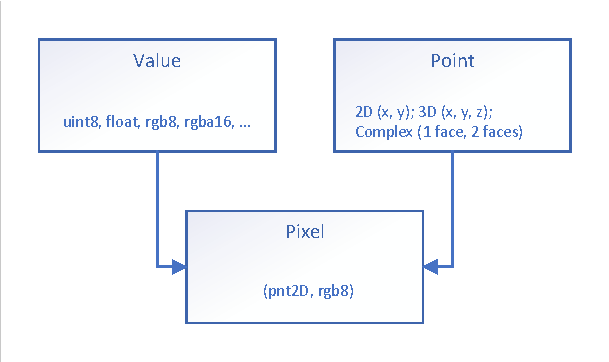
\includegraphics[width=.5\linewidth]{figs/concepts/pixel.pdf}
  \caption{Pixel concept.}
  \label{fig:concept.pixel}
\end{figure}

\begin{figure}[tbh]
  \centering
  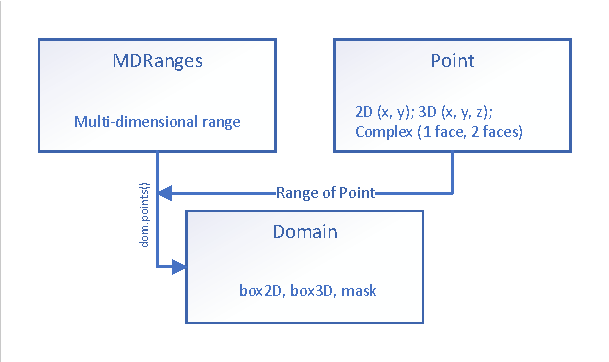
\includegraphics[width=.5\linewidth]{figs/concepts/domain.pdf}
  \caption{Domain concept.}
  \label{fig:concept.domain}
\end{figure}

\begin{figure}[tbh]
  \centering
  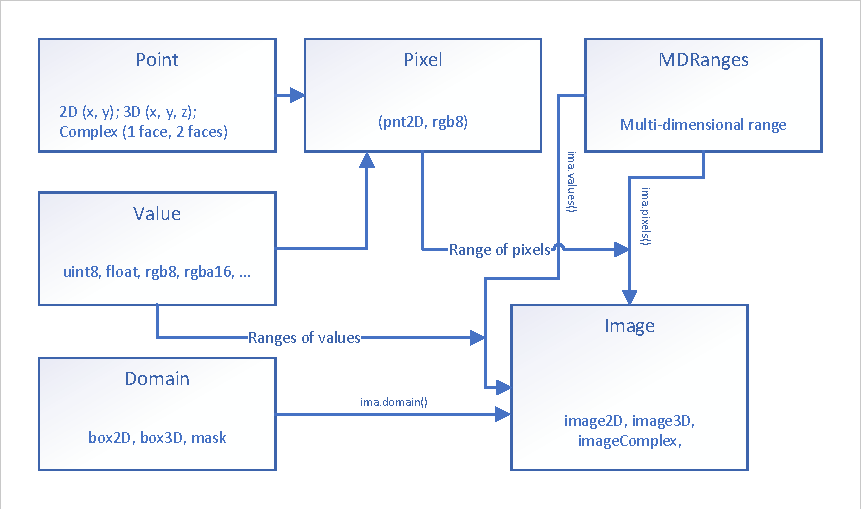
\includegraphics[width=.5\linewidth]{figs/concepts/image.pdf}
  \caption{Image concept.}
  \label{fig:concept.image}
\end{figure}

\begin{figure}[tbh]
  \centering
  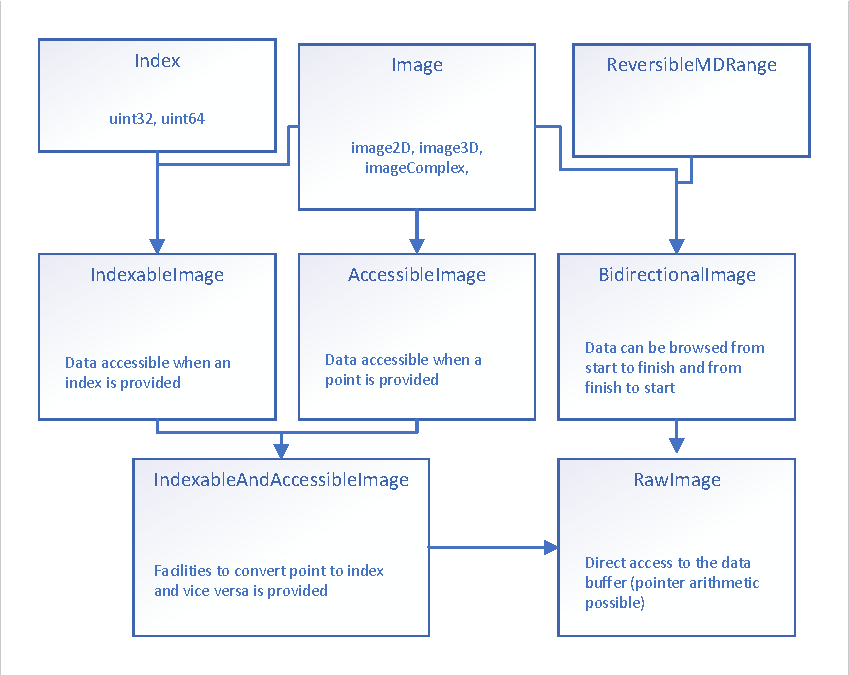
\includegraphics[width=.5\linewidth]{figs/concepts/images_all.pdf}
  \caption{All images concepts.}
  \label{fig:concept.images}
\end{figure}


\begin{figure}[tbh]
  \centering
  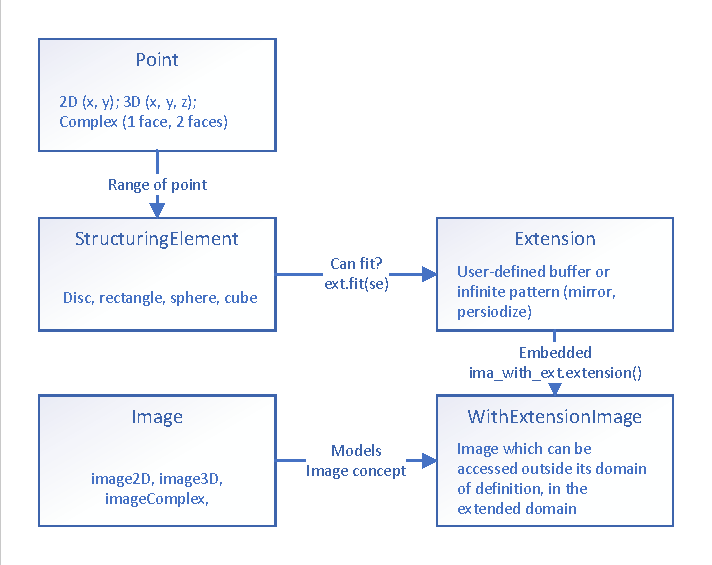
\includegraphics[width=.5\linewidth]{figs/concepts/se_extension.pdf}
  \caption{Structuring element and Extension concepts.}
  \label{fig:concept.se_extension}
\end{figure}

Let us now delve into concepts related to the Image Processing area. Indeed, this domain has his specificities and we
want to improve generic image processing library design by learning from our past experiments and working with new
techniques. The most basic usage of an image is the famous algebraic formula $y = f(x)$ where $y$ is a \emph{value}
generated by the \emph{image} $f$ for the \emph{emph} $x$. Aside from generating a value, an image can also \emph{store}
a value, as in $f(x) = y$ where the value is $assigned$ to the image for a given point. Those notions are the basis of
our work and will drive the entire design.

\subsection{The fundamentals}

\label{subsec:fundamentals}

First, let us introduce the fundamental concepts deriving from the basis notion. The \emph{Value} concept is refined
into three distincts one in~\cref{table:concept.value.expressions}. There are the basic \emph{Value} but also the
\emph{ComparableValue} and the \emph{OrderedValue} which are useful when it comes to comparison or ordering algorithms.

\begin{table}[!htbp]
  \begin{scriptsize}
    \begin{tabular}{llll}
      \cline{1-4}
      \thead{Concept} & \thead{Modeling type} & \thead{Inherit behavior from} & \thead{Instance of type}      \\
      \cline{1-4}
      Value           & \texttt{Val}          & $\emptyset$                   & \texttt{val}                  \\
      ComparableValue & \texttt{CmpVal}       & Value                         & \texttt{cmp\_val1, cmp\_val2} \\
      OrderedValue    & \texttt{OrdVal}       & ComparableValue               & \texttt{ord\_val1, ord\_val2} \\
      \cline{1-4}
    \end{tabular}
    \smallskip

    \begin{tabular}{llll}
      \cline{1-4}
      \thead{Concept}                                       & \thead{Expression}                                                   & \thead{Return
      Type}                                                 & \thead{Description}                                                                     \\
      \cline{1-4}
      \multicolumn{1}{c|}{Value}                            & \texttt{std::semiregular<Val>}                                       &
      \texttt{std::true\_type}                              & \makecell[l]{\texttt{Val} is a semiregular type. It can be:                             \\
      copied, moved, swapped,                                                                                                                         \\ and default constructed.}                                                                                                    \\
      \cline{1-4}
      \multicolumn{1}{c|}{\multirow{2}{*}{ComparableValue}} & \texttt{std::regular<CmpVal>}                                        &
      \texttt{std::true\_type}                              & \makecell[l]{\texttt{CmpVal} is a regular type. It is a semiregular                     \\
      type that is equality comparable.}                                                                                                              \\
      \multicolumn{1}{c|}{}                                 & \texttt{cmp\_val1 == cmp\_val2}                                      & \texttt{boolean}
                                                            & Supports equality comparison                                                            \\
      \cline{1-4}
      \multicolumn{1}{c|}{\multirow{2}{*}{OrderedValue}}    & \texttt{std::totally\_ordered<OrdVal>}                               &
      \texttt{std::true\_type}                              & \makecell[l]{\texttt{CmpVal} is a totally ordered as well as                            \\
      a regular type. Additionally the expressions                                                                                                    \\ must be equality preserving.}                                                                                           \\
      \multicolumn{1}{c|}{}                                 & \texttt{ord\_val1 < ord\_val2}                                       & \texttt{boolean}
                                                            & \multicolumn{1}{l}{\multirow{2}{*}{Supports inequality comparisons}}                    \\
      \multicolumn{1}{c|}{}                                 & \texttt{ord\_val1 <= ord\_val2, \dots}                               & \texttt{boolean}
                                                            & \multicolumn{1}{l}{}                                                                    \\
      \cline{1-4}
    \end{tabular}
    \smallskip

    \caption{Concepts Value: expressions}
  \end{scriptsize}
  \label{table:concept.value.expressions}
\end{table}

Then we have the concept of \emph{Point}, detailed in~\cref{table:concept.point.expressions} which is a bit more
constrained as it must be totally ordered. Indeed, when accessing a value stored in an image, wether it be reading of
mutating, it is important that there is only one accessed value.

\begin{table}[!htbp]
  \begin{scriptsize}
    \begin{tabular}{llll}
      \cline{1-4}
      \thead{Concept} & \thead{Modeling type} & \thead{Inherit behavior from} & \thead{Instance of type} \\
      \cline{1-4}
      Point           & \texttt{Pnt}          & $\emptyset$                   & \texttt{pnt1, pnt2}      \\
      \cline{1-4}
    \end{tabular}
    \smallskip

    \begin{tabular}{llll}
      \cline{1-4}
      \thead{Concept}                             & \thead{Expression}                     & \thead{Return Type}      &
      \thead{Description}                                                                                               \\
      \cline{1-4}
      \multicolumn{1}{c|}{\multirow{4}{*}{Point}} & \texttt{std::regular<Pnt>}             & \texttt{std::true\_type} &
      \makecell[l]{\texttt{Pnt} is a regular type. It can be:                                                           \\ copied, moved, swapped, and default
      constructed.                                                                                                      \\ It also is equality comparable.} \\
      \multicolumn{1}{c|}{}                       & \texttt{std::totally\_ordered<OrdVal>} & \texttt{std::true\_type} &
      \makecell[l]{\texttt{Pnt} is a totally ordered as well as a regular type.                                         \\ Additionally the expressions must be \\
      equality preserving.}                                                                                             \\
      \multicolumn{1}{c|}{}                       & \texttt{pnt1 < pnt2}                   & \texttt{boolean}         &
      \multicolumn{1}{l}{\multirow{2}{*}{supports inequality comparisons}}                                              \\
      \multicolumn{1}{c|}{}                       & \texttt{pnt1 <= pnt2, \dots}           & \texttt{boolean}         &
      \multicolumn{1}{l}{}                                                                                              \\
      \cline{1-4}
    \end{tabular}
    \smallskip

    \caption{Concepts Point: expressions}
  \end{scriptsize}
  \label{table:concept.point.expressions}
\end{table}

Now we introduce an abstract way to represent this relation $Value * Point$: the Pixel. This is a well known notion in
image processing and it represent a couple $(point, value)$. This facility is easy to move around and contains
facilities to read and mutate the pixel's value if possible. Indeed, not all pixel are able to mutate their value. If
the pixel is yielded by an image that only generate values on the fly then it cannot be mutated. Henceforth, we
introduce two new concepts: \emph{Pixel} and \emph{OutputPixel} in~\cref{table:concept.pixel.definitions}.

\begin{table}[!htbp]
  \begin{scriptsize}
    \begin{tabular}{llll}
      \cline{1-4}
      \thead{Concept} & \thead{Modeling type} & \thead{Inherit behavior from} & \thead{Instance of type} \\
      \cline{1-4}
      Pixel           & \texttt{Pix}          & $\emptyset$                   & \texttt{pix}             \\
      OutputPixel     & \texttt{OPix}         & Pixel                         & \texttt{opix}            \\
      \cline{1-4}
    \end{tabular}
    \smallskip

    \begin{tabular}{llll}
      \cline{1-4}
      \thead{Concept}                             & \thead{Definition}       & \thead{Description}            &
      \thead{Requirement}                                                                                       \\
      \cline{1-4}
      \multicolumn{1}{c|}{\multirow{3}{*}{Pixel}} & \texttt{value\_type}     & \makecell[l]{Type of the value
      contained in the pixel.                                                                                   \\ Cannot be constant or reference.}       & Models
      the concept \texttt{Value}.                                                                               \\
      \multicolumn{1}{c|}{}                       & \texttt{reference\_type} & \makecell[l]{Type used to
      mutate the pixel's value                                                                                  \\ if non-const. Can be a proxy.}       & \makecell[l]{Models the concept \\
      \texttt{std::indirectly\_writable} if non-const.}                                                         \\
      \multicolumn{1}{c|}{}                       & \texttt{point\_type}     & Type of the pixel's point.     &
      Models the concept \texttt{Point}                                                                         \\
      \cline{1-4}
    \end{tabular}
    \smallskip

    \caption{Concepts Pixel: definitions}
  \end{scriptsize}
  \label{table:concept.pixel.definitions}
\end{table}

Those two concepts have a very similar interface described in~\cref{table:concept.pixel.expressions}. They can both
access the stored informations: the point and the value. On top of that, the \emph{OutputPixel} can mutate the value.


\begin{table}[!htbp]
  \begin{scriptsize}
    \begin{tabular}{ll}
      \cline{1-2}
      \thead{Type}              & \thead{Instance of type} \\
      \cline{1-2}
      \texttt{Pix::value\_type} & \texttt{val}             \\
      \texttt{Pix::point\_type} & \texttt{pnt}             \\
      \cline{1-2}
    \end{tabular}
    \smallskip

    \begin{tabular}{llll}
      \cline{1-4}
      \thead{Concept}                             & \thead{Expression}        & \thead{Return Type}           &
      \thead{Description}                                                                                              \\
      \cline{1-4}
      \multicolumn{1}{c|}{\multirow{3}{*}{Pixel}} & \texttt{pix.val()}        & \texttt{Pix::reference\_type} &
      \makecell[l]{Access the pixel's value for read and/or write purpose.}                                            \\
      \multicolumn{1}{c|}{}                       & \texttt{pix.point()}      & \texttt{Pix::point\_type}     &
      \makecell[l]{Read the pixel's point.}                                                                            \\
      \multicolumn{1}{c|}{}                       & \texttt{pix.shift(pnt)}   & \texttt{void}                 & Shift
      pixel's point coordinate base on \texttt{pnt}'s coordinates.                                                     \\
      \cline{1-4}
      \multicolumn{1}{c|}{OutputPixel}            & \texttt{opix.val() = val} & \texttt{void}                 & Mutate
      pixel's value.                                                                                                   \\
      \cline{1-4}
    \end{tabular}
    \smallskip

    \caption{Concepts Pixel: expressions}
  \end{scriptsize}
  \label{table:concept.pixel.expressions}
\end{table}

Now we need a helper concept: the ranges.
Ranges~\parencite{niebler.2014.ranges,niebler.2018.ranges,niebler.2018.deepranges,niebler.2018.mergingranges} are a set
of concepts defined in the C++ standard library shipped with the ISO C++20 norm in 2020~\parencite{iso.2020.cpp}. They
allow the user to abstract away iterators to only iterate over one object: the range. This allow the user to migrate his
source code from:
\begin{minted}{C++}
template <class IteratorBegin, class IteratorEnd>
void my_algorithm(IteratorBegin beg, IteratorEnd end)
{
  for(; beg != end; ++beg)
    // ...
}
\end{minted}
To:
\begin{minted}{C++}
template <class Range>
void my_algorithm(Range rng)
{
  for(auto e : rng)
    // ...
}
\end{minted}

In image processing, we refine further this concept by introducing multi-dimensional ranges (\emph{MDRange}). Indeed, in
image processing the user is used to write double loop to iterate over a bi-dimensional image. And abstracting away this
aspect under standard ranges induce performance loss. That is why we needed this concept to exist. A multi-dimentional
range can be split with a library function, \texttt{mln::ranges::rows(mdrng)} to fit the double-loop pattern and keep
its performance. This topic is tackle in-depth later in~\cref{sec.range.traversing}. For now, let us consider
multi-dimensional ranges as an image processing extension for performance. They are defined
in~\cref{table:concept.ranges.definitions} and their interface is the same as standard ranges, as seen
in~\cref{table:concept.ranges.expressions}.

\begin{table}[!htbp]
  \begin{scriptsize}
    \begin{tabular}{llll}
      \cline{1-4}
      \thead{Concept}   & \thead{Modeling type} & \thead{Inherit behavior from} & \thead{Instance of type} \\
      \cline{1-4}
      MDRange           & \texttt{MDRng}        & $\emptyset$                   & \texttt{mdrng}           \\
      OutputMDRange     & \texttt{OMDRng}       & MDRange                       & \texttt{omdrng}          \\
      ReversibleMDRange & \texttt{RMDRng}       & MDRange                       & \texttt{rmdrng}          \\
      \cline{1-4}
    \end{tabular}
    \smallskip

    \begin{tabular}{llll}
      \cline{1-4}
      \thead{Concept}                               & \thead{Definition}       & \thead{Description}                      &
      \thead{Requirement}                                                                                                   \\
      \cline{1-4}
      \multicolumn{1}{c|}{\multirow{2}{*}{MDRange}} & \texttt{value\_type}     & \makecell[l]{Type of the value contained
      in the range.                                                                                                         \\ Cannot be constant or reference.} &  Models the concept \texttt{Value}. \\
      \multicolumn{1}{c|}{}                         & \texttt{reference\_type} & \makecell[l]{Type used to mutate the
      pixel's value                                                                                                         \\if non-const.                                                                                            Can be a proxy.}    & \makecell[l]{Models the concept \\
      \texttt{std::indirectly\_writable} if non-const.}                                                                     \\
      \cline{1-4}
    \end{tabular}

    \smallskip

    \caption{Concepts Ranges: definitions}
  \end{scriptsize}
  \label{table:concept.ranges.definitions}
\end{table}

\begin{table}[!htbp]
  \begin{scriptsize}
    \begin{tabular}{ll}
      \cline{1-2}
      \thead{Type}                                 & \thead{Instance of type} \\
      \cline{1-2}
      \texttt{std::ranges::range\_value\_t<MDRng>} & \texttt{val}             \\
      \cline{1-2}
    \end{tabular}
    \smallskip

    \begin{tabular}{llll}
      \cline{1-4}
      \thead{Concept}                                         & \thead{Expression}                              &
      \thead{Return Type}                                     & \thead{Description}                                                                            \\
      \cline{1-4}
      \multicolumn{1}{c|}{\multirow{2}{*}{MDRange}}           & \texttt{mdrng.begin()}                          &
      \texttt{unspecified}                                    & \makecell[l]{Return a forward iterator allowing                                                \\ a traversing of the range.} \\
      \multicolumn{1}{c|}{}                                   & \texttt{mdrng.end()}                            &
      \texttt{unspecified}                                    & \makecell[l]{Return a sentinel allowing to                                                     \\know when the end is reached.} \\
      \cline{1-4}
      \multicolumn{1}{c|}{OutputMDRange}                      & \makecell[l]{\texttt{auto it = omdrng.begin()}                                                 \\
      \texttt{*it++ = val}}                                   & \texttt{void}                                   & \makecell[l]{Mutate a value inside the range \\
      then increment the iterator's position}                                                                                                                  \\
      \cline{1-4}
      \multicolumn{1}{c|}{\multirow{2}{*}{ReversibleMDRange}} & \texttt{rmdrng.rbegin()}                        &
      \texttt{unspecified}                                    & \makecell[l]{Return a forward iterator allowing                                                \\ a traversing of the range \\ starting from
      the end.}                                                                                                                                                \\
      \multicolumn{1}{c|}{}                                   & \texttt{rmdrng.rend()}                          &
      \texttt{unspecified}                                    & \makecell[l]{Return a sentinel allowing to                                                     \\ know when the end is reached.} \\
      \cline{1-4}
    \end{tabular}
    \smallskip

    \caption{Concepts Ranges: expressions}
  \end{scriptsize}
  \label{table:concept.ranges.expressions}
\end{table}


From an algebraic point of view, the definition of an image is not complete without considering a definition domain on
which it is defined. In image processing, the same rule applies. We cannot consider an image without considering the set
of points that are valid for this image. Henceforth we must define the concept of \emph{Domain}
in~\emph{table:concept.domain.definitions}.

\begin{table}[!htbp]
  \begin{scriptsize}
    \begin{tabular}{llll}
      \cline{1-4}
      \thead{Concept} & \thead{Modeling type} & \thead{Inherit behavior from} & \thead{Instance of type} \\
      \cline{1-4}
      Domain          & \texttt{MDRng}        & MDRange                       & \texttt{dom}             \\
      SizedDomain     & \texttt{OMDRng}       & Domain                        & \texttt{sdom}            \\
      ShapedDomain    & \texttt{RMDRng}       & SizedDomain                   & \texttt{shdom}           \\
      \cline{1-4}
    \end{tabular}
    \smallskip

    \caption{Concepts Domain: definitions}
    \label{table:concept.domain.definitions}
  \end{scriptsize}
\end{table}

The \emph{Domain} concept is refined into two sub-concepts which are \emph{SizedDomain} and \emph{ShapedDomain}. This
emphasis the possibility of existence of possible infinite domain and domains that may be defined over non-continuous
intervals in space. This allows algorithms to requires the domain to have certain shape if needed. The domain behavior
is described in~\cref{table:concept.domain.expressions}

\begin{table}[!htbp]
  \begin{scriptsize}
    \begin{tabular}{ll}
      \cline{1-2}
      \thead{Type}              & \thead{Instance of type} \\
      \cline{1-2}
      \texttt{Dom::value\_type} & \texttt{pnt}             \\
      \cline{1-2}
    \end{tabular}
    \smallskip

    \begin{tabular}{llll}
      \cline{1-4}
      \thead{Concept}                              & \thead{Expression}               & \thead{Return Type}          &
      \thead{Description}                                                                                              \\
      \cline{1-4}
      \multicolumn{1}{c|}{\multirow{4}{*}{Domain}} & \texttt{Point<Dom::value\_type>} & \texttt{std::true\_type}     &
      \makecell[l]{Domain's value models the \texttt{Point} concept}                                                   \\
      \multicolumn{1}{c|}{}                        & \texttt{dom.has(pnt)}            & \texttt{bool}                &
      \makecell[l]{Check if a points is included in the domain.}                                                       \\
      \multicolumn{1}{c|}{}                        & \texttt{dom.empty()}             & \texttt{void}                &
      \makecell[l]{Read the pixel's point.}                                                                            \\
      \multicolumn{1}{c|}{}                        & \texttt{dom.dim()}               & \texttt{void}                &
      Returns the domain's dimension.                                                                                  \\
      \cline{1-4}
      \multicolumn{1}{c|}{SizedDomain}             & \texttt{sdom.size()}             & \texttt{unsigned int}        &
      Returns the number of points inside the domain.                                                                  \\
      \cline{1-4}
      \multicolumn{1}{c|}{ShapedDomain}            & \texttt{shdom.extends()}         & \texttt{std::forward\_range} &
      \makecell[l]{Return a range that yields the number                                                               \\ of elements for each dimension.}
      \\
      \cline{1-4}
    \end{tabular}
    \smallskip

    \caption{Concepts Domain: expressions}
  \end{scriptsize}
  \label{table:concept.domain.expressions}
\end{table}

Now we have all the tools to introduce our main concept: \emph{Image}. As for \emph{Pixel}, we have the distinction over
image whose value can be mutated in a sub-concept named \emph{WritableImage}. These concepts are defined
in~\cref{table:concept.image.definitions.1}.

\begin{table}[!htbp]
  \begin{scriptsize}
    \begin{tabular}{llll}
      \cline{1-4}
      \thead{Concept} & \thead{Modeling type} & \thead{Inherit behavior from} & \thead{Instance of type} \\
      \cline{1-4}
      \makecell[l]{Image (InputImage,                                                                    \\ ForwardImage)}    & \texttt{Img}          & $\emptyset$                                                                  & \texttt{img}             \\
      WritableImage   & \texttt{WImg}         & Image                         & \texttt{wimg}            \\
      \cline{1-4}
    \end{tabular}
    \smallskip

    \begin{tabular}{llll}
      \cline{1-4}
      \thead{Concept}                               & \thead{Definition}          & \thead{Description}                            & \thead{Requirement}                 \\
      \cline{1-4}
      \multicolumn{1}{c|}{\multirow{117}{*}{Image}} & \texttt{pixel\_type}        & Type of the image's pixel.                     & Models the concept \texttt{Pixel}.  \\
      \multicolumn{1}{c|}{}                         & \texttt{point\_type}        & Type of the image's point.                     & Models the concept \texttt{Point}.  \\
      \multicolumn{1}{c|}{}                         & \texttt{value\_type}        & \makecell[l]{Type of the image's value.                                              \\ Cannot be constant or reference} & Models the concept \texttt{Value}. \\
      \multicolumn{1}{c|}{}                         & \texttt{domain\_type}       & Type of the image's domain.                    & Models the concept \texttt{Domain}. \\
      \multicolumn{1}{c|}{}                         & \texttt{reference}          & \makecell[l]{Type used to mutate an image                                            \\ pixel's value if non-const} & \makecell[l]{Models the concept \\ \texttt{std::indirectly\_writable} \\ if non-const.}                                   \\
      \multicolumn{1}{c|}{}                         & \texttt{concrete\_type}     & Image concrete type (that holds data).         & Models the concept \texttt{Image}.  \\
      \multicolumn{1}{c|}{}                         & \texttt{ch\_value\_type<V>} & \makecell{Facility to return a new image type.                                       \\ that casts the underlying \texttt{value\_type} \\into \texttt{V}} & Models the concept \texttt{Image}. \\
      \cline{1-4}
    \end{tabular}
    \smallskip

    \caption{Concepts Image: definitions (1)}
    \label{table:concept.image.definitions.1}
  \end{scriptsize}
\end{table}

In addition to this definition we can infer the behavior described in~\cref{table:concept.image.expressions.1}. There
are complicated requirements written in template metaprogramming code. But in the end it is just to requires the ranges
returned by the member functions \texttt{pixels()} and \texttt{values()} to iterate over element whose type are the same
as those declared in the parent image.

\begin{table}[!htbp]
  \begin{scriptsize}
    \begin{tabular}{llll}
      \cline{1-4}
      \thead{Concept}                                     & \thead{Expression}                          & \thead{Return Type}                         &
      \thead{Description}                                                                                                                                                                           \\
      \cline{1-4}
      \multicolumn{1}{c|}{\multirow{7}{*}{Image}}         & \texttt{img.concretize()}                   & \makecell[l]{\texttt{std::convertible\_to<}                                               \\\texttt{concrete\_type>}} & \makecell[l]{Return a concrete image \\ that holds data.} \\
      \multicolumn{1}{c|}{}                               & \texttt{img.ch\_value<V>()}                 & \makecell[l]{\texttt{std::convertible\_to<}                                               \\\texttt{ch\_value\_type<V> >}} & \makecell[l]{Return an image whose values \\ are casted to \texttt{V}.}  \\
      \multicolumn{1}{c|}{}                               & \texttt{img.domain()}                       & \makecell[l]{\texttt{std::convertible\_to<}                                               \\\texttt{domain\_type>}} & Return the image's domain.  \\
      \multicolumn{1}{c|}{}                               & \texttt{img.pixels()}                       & \multirow{2}{*}{\texttt{MDRange}}           & \makecell[l]{Return a range that yields     \\ all the image pixels.} \\
      \multicolumn{1}{c|}{}                               & \texttt{img.values()}                       &                                             & \makecell[l]{Return a range that yields     \\ all the image values.} \\
      \multicolumn{1}{c|}{}                               & \makecell[l]{\texttt{std::convertible\_to<}                                                                                             \\\texttt{std::ranges::ranges\_value\_t<} \\\texttt{decltype(img.pixels())>,} \\\texttt{pixel\_type>}} & \multirow{2}{*}{\texttt{std::true\_type}}     & \multirow{2}{*}{\makecell[l]{Ranges converts to compatible\\ element types.}} \\
      \multicolumn{1}{c|}{}                               & \makecell[l]{\texttt{std::convertible\_to<}                                                                                             \\\texttt{std::ranges::ranges\_value\_t<} \\\texttt{decltype(img.values())>,} \\\texttt{value\_type>}} &      &  \\
      \cline{1-4}
      \multicolumn{1}{c|}{\multirow{2}{*}{WritableImage}} & \texttt{wimg.values()}                      & \texttt{OutputMDRange}                      & \makecell[l]{Return a range that yields all \\ the image values (mutable).} \\
      \multicolumn{1}{c|}{}                               & \makecell[l]{\texttt{OutputPixel<}                                                                                                      \\\texttt{std::ranges::ranges\_value\_t<} \\\texttt{decltype(wimg.pixels())> >}} & \texttt{std::true\_type}     & \multirow{2}{*}{Ranges whose elements are mutable.} \\
      \cline{1-4}
    \end{tabular}
    \smallskip

    \caption{Concepts Image: expressions (1)}
  \end{scriptsize}
  \label{table:concept.image.expressions.1}
\end{table}

In addition, we introduce two facilities which are the member function \texttt{concretize()} and
\texttt{ch\_value<V>()}. The first is a way to turn a view into a concrete type. This will be seen more in-depth
in~\cref{chap:image_views}. The last is a way to cast values from one type to another. It forms a new image type whose
underlying values will be returned after being casted to a new value type.


\subsection{Advanced way to access image data}
\label{subsec:advanced}

Being able to iterate over ranges of pixels or values is good and all but we are still lacking fundamental facilities to
access an element directly from the image. First we need to define the concept of \emph{Index}
in~\cref{table:concept.index.expressions} which we will use afterwards.

\begin{table}[!htbp]
  \begin{scriptsize}
    \begin{tabular}{llll}
      \cline{1-4}
      \thead{Concept} & \thead{Modeling type} & \thead{Inherit behavior from} & \thead{Instance of type} \\
      \cline{1-4}
      Index           & \texttt{Idx}          & $\emptyset$                   & \texttt{idx, idy}        \\
      \cline{1-4}
    \end{tabular}
    \smallskip

    \begin{tabular}{llll}
      \cline{1-4}
      \thead{Concept}                             & \thead{Expression}                   & \thead{Return Type}      &
      \thead{Description}                                                                                             \\
      \cline{1-4}
      \multicolumn{1}{c|}{\multirow{2}{*}{Index}} & \texttt{std::signed\_integral<Idx>}  & \texttt{std::true\_type} &
      Idx is a signed integral arithmetic type                                                                        \\
      \multicolumn{1}{c|}{}                       & \texttt{idx + idy, idx - idy, \dots} & \texttt{Idx}             &
      Supports all trivial arithmetical operations                                                                    \\
      \cline{1-4}
    \end{tabular}
    \smallskip

    \caption{Concepts Index: expressions}
  \end{scriptsize}
  \label{table:concept.index.expressions}
\end{table}

The first fundamental tool is represented as an \emph{IndexableImage}. An element can be accessed simply by providing
its index number. This concept is defined in~\cref{table:concept.image.definitions.2}.

\begin{table}[!htbp]
  \begin{scriptsize}
    \begin{tabular}{llll}
      \cline{1-4}
      \thead{Concept}        & \thead{Modeling type} & \thead{Inherit behavior from} & \thead{Instance of type} \\
      \cline{1-4}
      IndexableImage         & \texttt{IdxImg}       & Image                         & \texttt{idximg}          \\
      WritableIndexableImage & \texttt{WIdxImg}      & IndexableImage, WritableImage & \texttt{widximg}         \\
    \end{tabular}
    \smallskip

    \begin{tabular}{llll}
      \cline{1-4}
      \thead{Concept}                     & \thead{Definition}   & \thead{Description}               & \thead{Requirement}                \\
      \cline{1-4}
      \multicolumn{1}{c|}{IndexableImage} & \texttt{index\_type} & Type of the image's buffer index. & Models the concept \texttt{Index}. \\
      \cline{1-4}
    \end{tabular}
    \smallskip

    \caption{Concepts Image: definitions (2)}
    \label{table:concept.image.definitions.2}
  \end{scriptsize}
\end{table}

This introduces a simple behavioral pattern described in~\cref{table:concept.image.expressions.2}.

\begin{table}[!htbp]
  \begin{scriptsize}
    \begin{tabular}{lll}
      \cline{1-2}
      \thead{Type}                 & \thead{Instance of type} \\
      \cline{1-2}
      \texttt{Img::value\_type}    & \texttt{val}             \\
      \texttt{IdxImg::index\_type} & \texttt{k}               \\
      \cline{1-2}
    \end{tabular}
    \smallskip

    \begin{tabular}{llll}
      \cline{1-4}
      \thead{Concept}                     & \thead{Expression} & \thead{Return Type}               &
      \thead{Description}                                                                                                                           \\
      \cline{1-4}
      \multicolumn{1}{c|}{IndexableImage} & \texttt{idximg[k]} & \texttt{std::same\_as<reference>} & \makecell[l]{Access a value at a given index.} \\
      \cline{1-4}
      \multicolumn{1}{c|}{\makecell[l]{Writable                                                                                                     \\IndexableImage}} & \texttt{widximg[k] = val}                            & \texttt{void}                      & \makecell[l]{Mutate a value at a given index.} \\
      \cline{1-4}
    \end{tabular}
    \smallskip

    \caption{Concepts Image: expressions (2)}
  \end{scriptsize}
  \label{table:concept.image.expressions.2}
\end{table}

Additionally we want to be able to access a value by providing a point, the same way as in the algebraic definition $val = image(point)$.
To do so, we introduce the concept of accessibility through \emph{AccessibleImage}. This concept is defined in~\cref{table:concept.image.definitions.3}.

\begin{table}[!htbp]
  \begin{scriptsize}
    \begin{tabular}{llll}
      \cline{1-4}
      \thead{Concept}         & \thead{Modeling type} & \thead{Inherit behavior from}  & \thead{Instance of type} \\
      \cline{1-4}
      AccessibleImage         & \texttt{AccImg}       & Image                          & \texttt{accimg}          \\
      WritableAccessibleImage & \texttt{WAccImg}      & AccessibleImage, WritableImage & \texttt{waccimg}         \\
      \cline{1-4}
    \end{tabular}
    \smallskip

    \caption{Concepts Image: definitions (3)}
    \label{table:concept.image.definitions.3}
  \end{scriptsize}
\end{table}

This introduces new behavior that is described in~\cref{table:concept.image.expressions.3}. We can notice facilities
specifically including bound checking. Indeed, we suppose, for fast access, that the user is always picking element from
the image's domain but it is possible to bound check elements if needed on access for specific usages.

\begin{table}[!htbp]
  \begin{scriptsize}
    \begin{tabular}{lll}
      \cline{1-2}
      \thead{Type}              & \thead{Instance of type} \\
      \cline{1-2}
      \texttt{Img::point\_type} & \texttt{pnt}             \\
      \cline{1-2}
    \end{tabular}
    \smallskip

    \begin{tabular}{llll}
      \cline{1-4}
      \thead{Concept}                                       & \thead{Expression}                          & \thead{Return Type}                 &
      \thead{Description}                                                                                                                                                                         \\
      \cline{1-4}
      \multicolumn{1}{c|}{\multirow{4}{*}{AccessibleImage}} & \texttt{accimg(pnt)}                        & \texttt{std::same\_as<reference>}   & \makecell[l]{Access a value for a given point.} \\
      \multicolumn{1}{c|}{}                                 & \texttt{accimg.at(pnt)}                     & \texttt{std::same\_as<reference>}   & \makecell[l]{Access a value for a given point.  \\ No bound checking.} \\
      \multicolumn{1}{c|}{}                                 & \texttt{accimg.pixel(pnt)}                  & \texttt{std::same\_as<pixel\_type>} & \makecell[l]{Access a pixel for a given point.} \\
      \multicolumn{1}{c|}{}                                 & \texttt{accimg.pixel\_at(pnt)}              & \texttt{std::same\_as<pixel\_type>} & \makecell[l]{Access a pixel for a given point.  \\ No bound checking.} \\
      \cline{1-4}
      \multicolumn{1}{c|}{\multirow{4}{*}{\makecell[l]{Writable                                                                                                                                   \\AccessibleImage}}} & \texttt{img(pnt) = val}                            & \texttt{void}                      & \makecell[l]{Mutate a value at a given point.} \\
      \multicolumn{1}{c|}{}                                 & \texttt{waccimg.at(pnt) = val}              & \texttt{void}                       & \makecell[l]{Mutate a value at a given point.   \\ No bound checking.} \\
      \multicolumn{1}{c|}{}                                 & \makecell[l]{\texttt{OutputPixel<decltype(}                                                                                         \\\texttt{waccimg.pixel(pnt))>}}                            & \texttt{std::true\_type}                      & \makecell[l]{The returned pixel \\ models \texttt{OutputPixel}.} \\
      \multicolumn{1}{c|}{}                                 & \makecell[l]{\texttt{OutputPixel<decltype(}                                                                                         \\\texttt{waccimg.pixel\_at(pnt))>}}                            & \texttt{std::true\_type}                      & \makecell[l]{The returned pixel \\ models \texttt{OutputPixel}. \\ No bound checking.} \\
      \cline{1-4}
    \end{tabular}
    \smallskip

    \caption{Concepts Image: expressions (3)}
  \end{scriptsize}
  \label{table:concept.image.expressions.3}
\end{table}

Once we know that an image is both \emph{indexable} and \emph{accessible} we can deduce new behaviors (described
in~\cref{table:concept.image.expressions.4}) that we put behind the concept of \emph{IndexableAndAccessibleImage}
defined in~\emph{table:concept.image.definitions.4}. This behavior is related to accessing index from points and vise
versa.

\begin{table}[!htbp]
  \begin{scriptsize}
    \begin{tabular}{llll}
      \cline{1-4}
      \thead{Concept} & \thead{Modeling type} & \thead{Inherit behavior from} & \thead{Instance of type} \\
      \makecell[l]{IndexableAnd                                                                          \\ AccessibleImage}         & \texttt{IdxAccImg}    & IndexableImage, AccessibleImage                                              & \texttt{idxaccimg}       \\
      \makecell[l]{ WritableIndexable                                                                    \\ AndAccessibleImage} & \texttt{WIdxAccImg}   & \makecell[l]{IndexableAndAccessibleImage, \\ WritableIndexableImage, \\WritableAccessibleImage} & \texttt{widxaccimg}      \\
      \cline{1-4}
    \end{tabular}
    \smallskip

    \caption{Concepts Image: definitions (4)}
    \label{table:concept.image.definitions.4}
  \end{scriptsize}
\end{table}

\begin{table}[!htbp]
  \begin{scriptsize}
    \begin{tabular}{llll}
      \cline{1-4}
      \thead{Concept}       & \thead{Expression}                       & \thead{Return Type}  &
      \thead{Description}                                                                                                                    \\
      \cline{1-4}
      \multicolumn{1}{c|}{\multirow{3}{*}{\makecell[l]{IndexableAnd                                                                          \\AccessibleImage}}} & \texttt{img.point\_at\_index(k)}                            & \texttt{point\_type}                      & \makecell[l]{Get the point corresponding\\ to the given index.} \\
      \multicolumn{1}{c|}{} & \texttt{idxaccimg.index\_of\_point(pnt)} & \texttt{index\_type} & \makecell[l]{Get the linear index (offset in \\ the buffer) of multi-dimensional point.} \\
      \multicolumn{1}{c|}{} & \texttt{idxaccimg.delta\_index(pnt)}     & \texttt{index\_type} & \makecell[l]{Get the linear index offset     \\ for the given point.} \\
      \cline{1-4}
    \end{tabular}
    \smallskip

    \caption{Concepts Image: expressions (4)}
  \end{scriptsize}
  \label{table:concept.image.expressions.4}
\end{table}

Additionally we assume that an image can be traversed in a forward way as well as in a backward way. This may not be
true for all images so this notion needs to be refined into a new concept \emph{BidirectionalImage}. This concept is
defined in~\cref{table:concept.image.definitions.5} and its behavior is described
in~\cref{table:concept.image.expressions.5}.

\begin{table}[!htbp]
  \begin{scriptsize}
    \begin{tabular}{llll}
      \cline{1-4}
      \thead{Concept}            & \thead{Modeling type} & \thead{Inherit behavior from}     & \thead{Instance of type} \\
      \cline{1-4}
      BidirectionalImage         & \texttt{BidirImg}     & Image                             & \texttt{bidirimg}        \\
      WritableBidirectionalImage & \texttt{WBidirImg}    & BidirectionalImage, WritableImage & \texttt{wbidirimg}       \\
      \cline{1-4}
    \end{tabular}
    \smallskip

    \caption{Concepts Image: definitions (5)}
    \label{table:concept.image.definitions.5}
  \end{scriptsize}
\end{table}

\begin{table}[!htbp]
  \begin{scriptsize}
    \begin{tabular}{lll}
      \cline{1-2}
      \thead{Type}                 & \thead{Instance of type} \\
      \cline{1-2}
      \texttt{Img::point\_type}    & \texttt{pnt}             \\
      \texttt{Img::value\_type}    & \texttt{val}             \\
      \texttt{IdxImg::index\_type} & \texttt{k}               \\
      \texttt{int}                 & \texttt{dim}             \\
      \cline{1-2}
    \end{tabular}
    \smallskip

    \begin{tabular}{llll}
      \cline{1-4}
      \thead{Concept}                                          & \thead{Expression}         & \thead{Return Type}                         &
      \thead{Description}                                                                                                                                                                      \\
      \cline{1-4}
      \multicolumn{1}{c|}{\multirow{2}{*}{BidirectionalImage}} & \texttt{bidirimg.pixels()} & \multirow{2}{*}{\texttt{ReversibleMDRange}} & \makecell[l]{Return a reversible range that yields \\ all the image pixels.} \\
      \multicolumn{1}{c|}{}                                    & \texttt{bidirimg.values()} &                                             & \makecell[l]{Return a reversible range that yields \\ all the image values.} \\
      \cline{1-4}
      \cline{1-4}
    \end{tabular}
    \smallskip

    \caption{Concepts Image: expressions (5)}
  \end{scriptsize}
  \label{table:concept.image.expressions.5}
\end{table}

Now we need a way, when possible, to iterate over a continuous data buffer for very fast and optimized
calculation. That is what the concept of \emph{RawImage} is for: an image whose data buffer can be accessed, as well as its
mutable counterpart. It is defined defined in~\cref{table:concept.image.definitions.6}.

\begin{table}[!htbp]
  \begin{scriptsize}
    \begin{tabular}{llll}
      \cline{1-4}
      \thead{Concept}  & \thead{Modeling type} & \thead{Inherit behavior from}                  & \thead{Instance of type} \\
      \cline{1-4}
      RawImage         & \texttt{RawImg}       & \makecell[l]{IndexableAndAccessibleImage,                                 \\BidirectionalImage}                              & \texttt{rawimg}          \\
      WritableRawImage & \texttt{WRawImg}      & \makecell[l]{RawImage, WritableIndexableImage,                            \\WritableBidirectionalImage}                 & \texttt{wrawimg}         \\
      \cline{1-4}
    \end{tabular}
    \smallskip

    \caption{Concepts Image: definitions (6)}
    \label{table:concept.image.definitions.6}
  \end{scriptsize}
\end{table}

Having a raw image whose data buffer can be accessed allow ust to expose two more member function to access the
data buffer and its strides for correct pointer arithmetic. They behave as described in~\cref{table:concept.image.expressions.6}.

\begin{table}[!htbp]
  \begin{scriptsize}
    \begin{tabular}{llll}
      \cline{1-4}
      \thead{Concept}                                & \thead{Expression}                   & \thead{Return Type}                         &
      \thead{Description}                                                                                                                                                                       \\
      \cline{1-4}
      \multicolumn{1}{c|}{\multirow{2}{*}{RawImage}} & \texttt{rawimg.data()}               & \makecell[l]{\texttt{std::convertible\_to<}                                                       \\\texttt{const value\_type*>}} & \makecell[l]{Get a constant pointer to \\ the first element of the domain.} \\
      \multicolumn{1}{c|}{}                          & \texttt{rawimg.stride(dim)}          & \texttt{std::ptrdiff\_t}                    & \makecell[l]{Get the stride (in number of elements) \\ between two consecutive elements \\in the given \texttt{dim}.} \\
      \cline{1-4}
      \multicolumn{1}{c|}{\multirow{2}{*}{\makecell[l]{Writable                                                                                                                                 \\RawImage}}}           & \texttt{img.data()}                         & \makecell[l]{\texttt{std::convertible\_to<}\\\texttt{value\_type*>}} & \makecell[l]{Get a pointer to the first\\ element of the domain.} \\
      \multicolumn{1}{c|}{}                          & \texttt{*(wrawimg.data() + k) = val} & \texttt{void}                               & \makecell[l]{Access an element from the data        \\buffer at index \texttt{k} and mutate it \\ to \texttt{val}.} \\
      \cline{1-4}
      \multicolumn{1}{c|}{\makecell[l]{WithExtension                                                                                                                                            \\Image}}           & \texttt{wextimg.extension()}                         & \makecell[l]{\texttt{std::convertible\_to<}\\\texttt{extension\_type>}} & \makecell[l]{Get the extension of the image.} \\
      \cline{1-4}
    \end{tabular}
    \smallskip

    \caption{Concepts Image: expressions (6)}
  \end{scriptsize}
  \label{table:concept.image.expressions.6}
\end{table}


\subsection{Local algorithm concepts: structuring elements and extensions}
\label{subsec:local.se.ext}


From the beginning concepts are emerging from behavioral patterns extracted from algorithms. In image processing, there
is a family of algorithms called the \emph{local algorithms}. They work by considering a specific pixel as well as all
the pixels among a window having a specific shape centered in this first pixel. The window is called the
\emph{structuring element} and the pixels considered by this window are called the \emph{neighborhood}. This leads us to
introduce the concept of \emph{StructuringElement} which is defined in~\cref{table:concept.se.definitions}.

\begin{table}[!htbp]
  \begin{scriptsize}
    \begin{tabular}{llll}
      \cline{1-4}
      \thead{Concept}                & \thead{Modeling type} & \thead{Inherit behavior from} & \thead{Instance of type} \\
      \cline{1-4}
      StructuringElement             & \texttt{SE, Pnt}      & $\emptyset$, Point            & \texttt{se, pnt}         \\
      DecomposableStructuringElement & \texttt{DSE, Pnt}     & StructuringElement, Point     & \texttt{dse}             \\
      SeparableStructuringElement    & \texttt{SSE, Pnt}     & StructuringElement, Point     & \texttt{sse}             \\
      IncrementalStructuringElement  & \texttt{ISE, Pnt}     & StructuringElement, Point     & \texttt{ise}             \\
      \cline{1-4}
    \end{tabular}
    \smallskip

    \begin{tabular}{llll}
      \cline{1-4}
      \thead{Concept}                                          & \thead{Definition}    & \thead{Description}                           &
      \thead{Requirement}                                                                                                                                                                                   \\
      \cline{1-4}
      \multicolumn{1}{c|}{\multirow{3}{*}{StructuringElement}} & \texttt{incremental}  & \multirow{3}{*}{\texttt{std::bool\_constant}} & \multirow{3}{*}{\makecell[l]{\texttt{std::true\_type} if supported \\ \texttt{std::false\_false} otherwise.}} \\
      \multicolumn{1}{c|}{}                                    & \texttt{decomposable} &                                               &                                                                    \\
      \multicolumn{1}{c|}{}                                    & \texttt{separable}    &                                               &                                                                    \\
      \cline{1-4}
    \end{tabular}
    \smallskip

    \caption{Concepts Structuring Elements: definitions}
    \label{table:concept.se.definitions}
  \end{scriptsize}
\end{table}

This concept is refined into three subconcepts that are related to properties the structuring element can offer. Those
properties are:
\begin{itemize}
  \item decomposability: ability to split a complex structuring element into several smaller and simpler structuring
        element. There is an equivalence in behavior when the algorithm is recursively run for each smaller structuring
        element one after another, in a multipass way.
  \item separability: ability to split a complex structuring element into several smaller and simpler structuring
        element. There is an equivalence in behavior when the convolution is recursively run for each smaller structuring
        element one after another, in a precise order, in a multipass way.
  \item incremental: ability to tell the points that are added to or removed from the range when the structuring element
        is shifted by a basic displacement (e.g. for a \emph{2D point}, the basic deplacement is $(0,1)$). Usually used to
        compute attributes over a sliding structuring element in linear time.
\end{itemize}
The behavioral for those concepts is discribed in~\cref{table:concept.se.expressions}.

\begin{table}[!htbp]
  \begin{scriptsize}
    \begin{tabular}{lll}
      \cline{1-3}
      \thead{Type} & \thead{Instance of type} & \thead{Requirement}                           \\
      \cline{1-3}
      \texttt{Pix} & \texttt{pix}             & \texttt{std::same\_as<Pix::point\_type, Pnt>} \\
      \texttt{Pnt} & \texttt{pnt}             &                                               \\
      \cline{1-3}
    \end{tabular}
    \smallskip

    \begin{tabular}{llll}
      \cline{1-4}
      \thead{Concept}                                           & \thead{Expression}                                    & \thead{Return Type}                       &
      \thead{Description}                                                                                                                                                                                     \\
      \cline{1-4}
      \multicolumn{1}{c|}{\multirow{11}{*}{StructuringElement}} & \multirow{2}{*}{\texttt{std::regular\_invocable<SE,
      Pnt>}}                                                    & \multirow{4}{*}{\texttt{std::true\_type}}             &
      \multirow{4}{*}{\makecell[l]{\texttt{se} can called using \text{std::invoke},                                                                                                                           \\ is equality preserving and \\
      does not modify function object                                                                                                                                                                         \\ nor arguments.}} \\
      \multicolumn{1}{c|}{}                                     &                                                       &
                                                                &                                                                                                                                             \\
      \multicolumn{1}{c|}{}                                     & \multirow{2}{*}{\texttt{std::regular\_invocable<SE,
      Pix>}}                                                    &                                                       &
      \\
      \multicolumn{1}{c|}{}                                     &                                                       &                                           &                                         \\
      \multicolumn{1}{c|}{}                                     & \texttt{se(pnt)}                                      & \texttt{std::forward\_range}              &
      \makecell[l]{Return a range that yeilds the                                                                                                                                                             \\
      neighboring points of \texttt{pnt}.}                                                                                                                                                                    \\
      \multicolumn{1}{c|}{}                                     & \texttt{se.offsets()}                                 & \texttt{std::forward\_range}              &
      \makecell[l]{Return a range that yeilds the                                                                                                                                                             \\
      neighboring points,                                                                                                                                                                                     \\in relative coordinates.}                                                                                                                                                          \\
      \multicolumn{1}{c|}{}                                     & \texttt{se(pix)}                                      & \texttt{std::forward\_range}              &
      \makecell[l]{Return a range that yeilds the                                                                                                                                                             \\
      neighboring pixels of \texttt{pix}.}                                                                                                                                                                    \\
      \multicolumn{1}{c|}{}                                     & \texttt{se.radial\_extent()}                          & \texttt{int}                              &
      \makecell[l]{Returns the radial extent                                                                                                                                                                  \\of the SE,
      the radius                                                                                                                                                                                              \\of the disc (square).}                                                                                                                                                                      \\
      \multicolumn{1}{c|}{}                                     & \makecell[l]{\texttt{std::convertible\_to<}                                                                                                 \\
      \texttt{std::ranges::range\_value\_t<}                                                                                                                                                                  \\ \texttt{decltype(se(pnt))>, Pnt>}}      &
      \multirow{3}{*}{\texttt{std::true\_type}}                 & \multirow{3}{*}{\makecell[l]{Converts to a compatible                                                                                       \\ point type}}
      \\
      \multicolumn{1}{c|}{}                                     & \makecell[l]{\texttt{std::convertible\_to<}                                                                                                 \\
      \texttt{std::ranges::range\_value\_t<}                                                                                                                                                                  \\ \texttt{decltype(se.offsets())>, Pnt>}} & & \\
      \multicolumn{1}{c|}{}                                     &
      \makecell[l]{\texttt{Pixel<std::ranges::range\_value\_t<}
      \\ \texttt{decltype(se(pix))> >}}                          &                                           & \makecell[l]{Is a range of compatible \\pixel type}                                                                                                                                                                \\
      \cline{1-4}
      \multicolumn{1}{c|}{\multirow{4}{*}{\makecell[l]{Decomposable                                                                                                                                           \\StructuringElement}}} & \texttt{dse.is\_decomposable()} & \texttt{std::bool\_constant} & \makecell[l]{\texttt{std::true\_type} if supported\\ \texttt{std::false\_false} otherwise.}\\
      \multicolumn{1}{c|}{}                                     & \texttt{dse.decompose()}                              & \texttt{std::forward\_range}              & \makecell[l]{Return a range that yeilds \\ simpler structuring elements.}\\
      \multicolumn{1}{c|}{}                                     & \makecell[l]{\texttt{StructuringElement<}                                                                                                   \\ \texttt{std::ranges::range\_value\_t<} \\ \texttt{decltype(dse.decompose())> >}}                            & \texttt{std::true\_type} & \makecell[l]{Is a range of compatible \\structuring elements types.}\\
      \multicolumn{1}{c|}{}                                     & \texttt{dse.is\_decomposable()}                       & \texttt{bool}                             & \makecell[l]{Wether the decompose       \\ facility is supported}\\
      \cline{1-4}
      \multicolumn{1}{c|}{\multirow{4}{*}{\makecell[l]{Separable                                                                                                                                              \\StructuringElement}}} & \texttt{dse.is\_decomposable()} & \texttt{std::bool\_constant} & \makecell[l]{\texttt{std::true\_type} if supported\\ \texttt{std::false\_false} otherwise.}\\
      \multicolumn{1}{c|}{}                                     & \texttt{sse.separate()}                               & \texttt{std::forward\_range}              & \makecell[l]{Return a range that yeilds \\ simpler structuring elements.}\\
      \multicolumn{1}{c|}{}                                     & \makecell[l]{\texttt{StructuringElement<}                                                                                                   \\ \texttt{std::ranges::range\_value\_t<} \\ \texttt{decltype(sse.separate())> >}}                            & \texttt{std::true\_type} & \makecell[l]{Is a range of compatible \\structuring elements types.}\\
      \multicolumn{1}{c|}{}                                     & \texttt{sse.is\_separable()}                          & \texttt{bool}                             & \makecell[l]{Wether the separate        \\ facility is supported}\\
      \cline{1-4}
      \multicolumn{1}{c|}{\multirow{4}{*}{\makecell[l]{Incremental                                                                                                                                            \\StructuringElement}}} & \texttt{dse.is\_decomposable()} & \texttt{std::bool\_constant} & \makecell[l]{\texttt{std::true\_type} if supported\\ \texttt{std::false\_false} otherwise.}\\
      \multicolumn{1}{c|}{}                                     & \texttt{ise.inc()}                                    & \makecell[l]{\texttt{StructuringElement<}                                           \\\texttt{SE, Pnt>}} & \makecell[l]{Return the next            \\ simpler structuring elements.}\\
      \multicolumn{1}{c|}{}                                     & \texttt{ise.dec()}                                    & \makecell[l]{\texttt{StructuringElement<}                                           \\\texttt{SE, Pnt>}} & \makecell[l]{Return the previous        \\ simpler structuring elements.}\\
      \multicolumn{1}{c|}{}                                     & \texttt{ise.is\_incremental()}                        & \texttt{bool}                             & \makecell[l]{Wether the incremental     \\ facility is supported}\\
      \cline{1-4}
    \end{tabular}
    \smallskip

    \caption{Concepts Structuring Elements: expressions}
  \end{scriptsize}
  \label{table:concept.se.expressions}
\end{table}

Additionally, we introduce the concept of \emph{Neighborhood} in~\cref{table:concept.nbh.definitions}. This concept has
facilities to know what points/pixels are placed before or after another point/pixel inside the window of a specific
structuring element. It behaves as described in~\cref{table:concept.nbh.expressions}.

\begin{table}[!htbp]
  \begin{scriptsize}
    \begin{tabular}{llll}
      \cline{1-4}
      \thead{Concept} & \thead{Modeling type} & \thead{Inherit behavior from} & \thead{Instance of type} \\
      \cline{1-4}
      Neighborhood    & \texttt{SE, Pnt}      & StructuringElement, Point     & \texttt{se, pnt}         \\
      \cline{1-4}
    \end{tabular}
    \smallskip

    \caption{Concepts Neighborhood: definitions}
    \label{table:concept.nbh.definitions}
  \end{scriptsize}
\end{table}

\begin{table}[!htbp]
  \begin{scriptsize}
    \begin{tabular}{lll}
      \cline{1-3}
      \thead{Type} & \thead{Instance of type} & \thead{Requirement}                           \\
      \cline{1-3}
      \texttt{Pix} & \texttt{pix}             & \texttt{std::same\_as<Pix::point\_type, Pnt>} \\
      \texttt{Pnt} & \texttt{pnt}             &                                               \\
      \cline{1-3}
    \end{tabular}
    \smallskip

    \begin{tabular}{llll}
      \cline{1-4}
      \thead{Concept}                                    & \thead{Expression}                          & \thead{Return Type}                           &
      \thead{Description}                                                                                                                                                                                           \\
      \cline{1-4}
      \multicolumn{1}{c|}{\multirow{8}{*}{Neighborhood}} & \texttt{se.before(pnt)}                     & \multirow{4}{*}{\texttt{std::forward\_range}} & Return a range that yields the points before \texttt{pnt}. \\
      \multicolumn{1}{c|}{}                              & \texttt{se.after(pnt)}                      &                                               & Return a range that yields the points after \texttt{pnt}.  \\
      \multicolumn{1}{c|}{}                              & \texttt{se.before(pix)}                     &                                               & Return a range that yields the pixels before \texttt{pix}. \\
      \multicolumn{1}{c|}{}                              & \texttt{se.after(pix)}                      &                                               & Return a range that yields the pixels after \texttt{pnt}.  \\
      \multicolumn{1}{c|}{}                              & \makecell[l]{\texttt{std::convertible\_to<}                                                                                                              \\\texttt{std::ranges::ranges\_value\_t<}\\\texttt{decltype(se.before(pnt))>, Pnt>}} & \multirow{4}{*}{\texttt{std::true\_type}}     & \multirow{2}{*}{Ranges converts to compatible element types.} \\
      \multicolumn{1}{c|}{}                              & \makecell[l]{\texttt{std::convertible\_to<}                                                                                                              \\\texttt{std::ranges::ranges\_value\_t<}\\\texttt{decltype(se.after(pnt))>, Pnt>}}  &                                               &                                                                    \\
      \multicolumn{1}{c|}{}                              & \makecell[l]{\texttt{Pixel<}                                                                                                                             \\\texttt{std::ranges::ranges\_value\_t<}\\\texttt{decltype(se.before(pix))>, Pix>}}                 &                                               & \multirow{2}{*}{Ranges that are of compatible element types.}      \\
      \multicolumn{1}{c|}{}                              & \makecell[l]{\texttt{Pixel<}                                                                                                                             \\\texttt{std::ranges::ranges\_value\_t<}\\\texttt{decltype(se.after(pix))>, Pix>}}                  &                                               &                                                                    \\
      \cline{1-4}
    \end{tabular}
    \smallskip

    \caption{Concepts Neighborhood: expressions}
  \end{scriptsize}
  \label{table:concept.nbh.expressions}
\end{table}

And the last side concept to introduce to our current galaxy is the extension. Indeed, extension management is very
important when dealing with local algorithm as pixels on the border need to be processed and the behavior near the
border of the image must be defined and well-specified. There are several strategies when it comes to borders and extension.
We refine concept for each strategy we identified:
\begin{itemize}
  \item fillable: fill the border with a specific value.
  \item mirrorable: mirror the image as if there was an axial symmetry, with the border being the axis.
  \item periodizeable: repeat the image, as if a modulo size wasa applied to the coordinates.
  \item clampable: extend the value at the image's border into the extension.
  \item extent with: used when tiling. it consider the current image as a subimage of another bigger image and pick the
        extension values there.
\end{itemize}
Those concepts are defined in~\cref{table:concept.extensions.definitions} and their behavior is described
in~\cref{table:concept.extensions.expressions}.

\begin{table}[!htbp]
  \begin{scriptsize}
    \begin{tabular}{llll}
      \cline{1-4}
      \thead{Concept}       & \thead{Modeling type}  & \thead{Inherit behavior from} & \thead{Instance of type} \\
      \cline{1-4}
      Extension             & \texttt{Ext, Pnt}      & $\emptyset$, Point            & \texttt{ext, pnt}        \\
      FillableExtension     & \texttt{FExt, Pnt}     & Extension, Point              & \texttt{fext}            \\
      MirrorableExtension   & \texttt{MExt, Pnt}     & Extension, Point              & \texttt{mext}            \\
      PeriodizableExtension & \texttt{PExt, Pnt}     & Extension, Point              & \texttt{pext}            \\
      ClampableExtension    & \texttt{CExt, Pnt}     & Extension, Point              & \texttt{cext}            \\
      ExtendWithExtension   & \texttt{EwExt, Pnt, U} & Extension, Point, Image       & \texttt{ewext, u}        \\
      \cline{1-4}
    \end{tabular}
    \smallskip

    \begin{tabular}{llll}
      \cline{1-4}
      \thead{Concept}                                 & \thead{Definition}                     & \thead{Description}                           &
      \thead{Requirement}                                                                                                                                                                                           \\
      \cline{1-4}
      \multicolumn{1}{c|}{\multirow{6}{*}{Extension}} & \texttt{value\_type}                   & \makecell[l]{Type of value
      contained                                                                                                                                                                                                     \\ in the range.                                                                                                                                                                             Cannot be \\ constant
      or reference.}                                  & Models the concept \texttt{Value}.                                                                                                                          \\
      \multicolumn{1}{c|}{}                           & \texttt{support\_fill}                 & \multirow{5}{*}{\texttt{std::bool\_constant}} & \multirow{5}{*}{\makecell[l]{\texttt{std::true\_type} if supported \\ \texttt{std::false\_false} otherwise.}} \\
      \multicolumn{1}{c|}{}                           & \texttt{support\_mirror}               &                                               &                                                                    \\
      \multicolumn{1}{c|}{}                           & \texttt{support\_periodize}            &                                               &                                                                    \\
      \multicolumn{1}{c|}{}                           & \texttt{support\_clamp}                &                                               &                                                                    \\
      \multicolumn{1}{c|}{}                           & \texttt{support\_extend\_with}         &                                               &                                                                    \\
      \cline{1-4}
      \multicolumn{1}{c|}{ExtendWithExtension}        & \texttt{point\_type}                   & \makecell[l]{Type of point in                                                                                      \\ the
      extended image.}                                & \makecell[l]{Converts to the sub-image                                                                                                                      \\ points type.}                                                                                                            \\
      \cline{1-4}
    \end{tabular}
  \end{scriptsize}
  \smallskip

  \caption{Concepts Extensions: definitions}
  \label{table:concept.extensions.definitions}
\end{table}

\begin{table}[!htbp]
  \begin{scriptsize}
    \begin{tabular}{ll}
      \cline{1-2}
      \thead{Type}              & \thead{Instance of type} \\
      \cline{1-2}
      \texttt{SE<Pnt, Pix>}     & \texttt{se}              \\
      \texttt{Ext::value\_type} & \texttt{val}             \\
      \texttt{Ext::point\_type} & \texttt{offset}          \\
      \cline{1-2}
    \end{tabular}
    \smallskip

    \begin{tabular}{llll}
      \cline{1-4}
      \thead{Concept}                                              & \thead{Expression}                            & \thead{Return Type} &
      \thead{Description}                                                                                                                                      \\
      \cline{1-4}
      \multicolumn{1}{c|}{\multirow{2}{*}{Extension}}              & \texttt{ext.fit(se)}                          & \texttt{bool}       & \makecell[l]{Wether
      the extension fit                                                                                                                                        \\ the structuring element.}                                                                                                   \\
      \multicolumn{1}{c|}{}                                        & \texttt{ext.extent()}                         & \texttt{int}        &
      \makecell[l]{Extension's border width.                                                                                                                   \\
      std::numeric\_limits<int>::max()                                                                                                                         \\ for infinite size.}                                                                                         \\
      \cline{1-4}
      \multicolumn{1}{c|}{\multirow{2}{*}{FillableExtension}}      & \texttt{fext.fill(val)}                       & \texttt{void}       &
      \makecell[l]{Fill the extension with                                                                                                                     \\the value \texttt{val}.}                                                                                              \\
      \multicolumn{1}{c|}{}                                        & \texttt{fext.is\_fill\_supported}             & \texttt{bool}       &
      \makecell[l]{Wether the fill facility                                                                                                                    \\is supported.}                                                                                                                            \\
      \cline{1-4}
      \multicolumn{1}{c|}{\multirow{2}{*}{MirrorableExtension}}    & \texttt{mext.mirror()}                        & \texttt{void}       & \makecell[l]{Fill
      the extension with                                                                                                                                       \\mirrored image's values.}                                                                                                  \\
      \multicolumn{1}{c|}{}                                        & \texttt{mext.is\_mirror\_supported()}         &
      \texttt{bool}                                                & \makecell[l]{Wether the mirror facility                                                   \\ is supported.}                                             \\
      \cline{1-4}
      \multicolumn{1}{c|}{\multirow{2}{*}{PeriodizeableExtension}} & \texttt{mext.periodize()}                     & \texttt{void}       &
      \makecell[l]{Fill the extension with                                                                                                                     \\periodic copies of image's values.}                                                                                   \\
      \multicolumn{1}{c|}{}                                        & \texttt{mext.is\_periodize\_supported()}      &
      \texttt{bool}                                                & \makecell[l]{Wether the mirror facility                                                   \\is supported.}                                      \\
      \cline{1-4}
      \multicolumn{1}{c|}{\multirow{2}{*}{ClampableExtension}}     & \texttt{mext.clamp()}                         & \texttt{void}       & \makecell[l]{Fill
      the extension by                                                                                                                                         \\extending image's values \\at extremities.}                                                                                    \\
      \multicolumn{1}{c|}{}                                        & \texttt{mext.is\_clamp\_supported()}          &
      \texttt{bool}                                                & \makecell[l]{Wether the clamp facility                                                    \\is supported.}                                       \\
      \cline{1-4}
      \multicolumn{1}{c|}{\multirow{3}{*}{ExtendWithExtension}}    &
      \makecell[l]{\texttt{std::convertible\_to<point\_type,}                                                                                                  \\\texttt{U::point\_type>}} & \texttt{std::true\_type} &
      \makecell[l]{Converts to the sub-image                                                                                                                   \\ points type.}                                                                                                       \\
      \multicolumn{1}{c|}{}                                        & \texttt{mext.extend\_with(u, offset)}         &
      \texttt{void}                                                & \makecell[l]{Fill the extension with                                                      \\sub-image      \texttt{u}'s values  starting \\ from \texttt{offset}.} \\
      \multicolumn{1}{c|}{}                                        & \texttt{mext.is\_extent\_with\_supported()}   &
      \texttt{bool}                                                & \makecell[l]{Wether the extend-with-sub-image                                             \\ facility is
      supported.}                                                                                                                                              \\
      \cline{1-4}
    \end{tabular}
    \smallskip

    \caption{Concepts Extensions: expressions}
  \end{scriptsize}
  \label{table:concept.extensions.expressions}
\end{table}


This allows us to introduce the final refined image concepts: \emph{WithExtensionImage} as well as \emph{ConcreteImage}
and \emph{ViewImage}. Those two last will be seen in detail in the next chapter~\ref{chap:image_views}. Those concepts
are defined in~\cref{table:concept.image.definitions.7}. Their behavior is described
in~\cref{table:concept.image.expressions.7}.

\begin{table}[!htbp]
  \begin{scriptsize}
    \begin{tabular}{llll}
      \cline{1-4}
      \thead{Concept}    & \thead{Modeling type} & \thead{Inherit behavior from} & \thead{Instance of type} \\
      \cline{1-4}
      WithExtensionImage & \texttt{WExtImg}      & Image                         & \texttt{wextimg}         \\
      ConcreteImage      & \texttt{CImg}         & Image                         & \texttt{cimg}            \\
      ViewImage          & \texttt{VImg}         & Image                         & \texttt{vimg}            \\
      \cline{1-4}
    \end{tabular}
    \smallskip

    \begin{tabular}{llll}
      \cline{1-4}
      \thead{Concept}                         & \thead{Definition}       & \thead{Description}            & \thead{Requirement}                    \\
      \cline{1-4}
      \multicolumn{1}{c|}{WithExtensionImage} & \texttt{extension\_type} & Type of the image's extension. & Models the concept \texttt{Extension}. \\
      \cline{1-4}
    \end{tabular}
    \smallskip

    \caption{Concepts Image: definitions (7)}
    \label{table:concept.image.definitions.7}
  \end{scriptsize}
\end{table}

\begin{table}[!htbp]
  \begin{scriptsize}
    \begin{tabular}{llll}
      \cline{1-4}
      \thead{Concept} & \thead{Expression} & \thead{Return Type} &
      \thead{Description}                                          \\
      \cline{1-4}
      \multicolumn{1}{c|}{\makecell[l]{WithExtension               \\Image}}           & \texttt{wextimg.extension()}                         & \makecell[l]{\texttt{std::convertible\_to<}\\\texttt{extension\_type>}} & \makecell[l]{Get the extension of the image.} \\
      \cline{1-4}
    \end{tabular}
    \smallskip

    \caption{Concepts Image: expressions (7)}
  \end{scriptsize}
  \label{table:concept.image.expressions.7}
\end{table}

Finally, we introduce a helper concept to centralize the detection of the "writability" of an image. Indeed, we do not
want the user to have to use the writable counterpart of each concept for each and every case. That is why we introduce
this final concept, \emph{OutputImage} in~\cref{table:concept.image.expressions.8}, that will tell the user if an image
is well-specified.

\begin{figure}[!htbp]
  \begin{scriptsize}
    \begin{equation}
      \begin{aligned}
        OutputImage ={} & (Image \implies WritableImage) \wedge                                             \\
                        & (IndexableImage \implies WritableIndexableImage) \wedge                           \\
                        & (AccessibleImage \implies WritableAccessibleImage) \wedge                         \\
                        & (IndexableAndAccessibleImage \implies WritableIndexableAndAccessibleImage) \wedge \\
                        & (BidirectionalImage \implies WritableBidirectionalImage) \wedge                   \\
                        & (RawImage \implies WritableRawImage)
      \end{aligned}
    \end{equation}
    \smallskip

    \caption{Concepts OutputImage: definition}
  \end{scriptsize}
  \label{table:concept.image.expressions.8}
\end{figure}

The correct way to use it is:
\begin{minted}{c++}
template <class Img>
requires RawImage<Img> && OutputImage<Img>
void my_algorithm(Img img) {
    // ...
  }
\end{minted}
